% Stage 1 report — compile with: tectonic main.tex (or any LaTeX distribution).
% Figures resolve from the repository's charts/ directory; on Overleaf, upload
% the charts/ tree next to main.tex (figures/ is also searched).
\documentclass[10pt,a4paper]{article}

\usepackage[utf8]{inputenc}
\usepackage[T1]{fontenc}
\usepackage{lmodern}
\usepackage[margin=2cm]{geometry}
% Allow slightly loose lines as a last resort instead of overflowing.
\setlength{\emergencystretch}{1.5em}
\usepackage{graphicx}
\usepackage{float}
\usepackage{booktabs}
\usepackage{tabularx}
\usepackage{longtable}
\usepackage{amsmath}
\usepackage{xcolor}
\usepackage{tikz}
\usetikzlibrary{arrows.meta,positioning,shapes.geometric}
\usepackage[colorlinks=true,linkcolor=blue!50!black,citecolor=blue!50!black,urlcolor=blue!50!black]{hyperref}
\usepackage{cleveref}

\graphicspath{{../charts/}{figures/}}

% Numbers fixed by code or by a completed run.
\newcommand{\fixed}[1]{\textcolor{black}{#1}}

\begin{document}

\begin{titlepage}
    \centering
    \vspace*{1cm}

    % Institution and Degree
    {\scshape\Large Universidad de Las Palmas de Gran Canaria \par}
    \vspace{0.5cm}
    {\scshape\large Grado en Ciencia e Ingeniería de Datos \par}
    \vspace{0.5cm}
    {\large Academic Year: 2026/2027 \par}
    \vspace{1cm}

    % Project title
    \IfFileExists{boogle-engine-logo.jpg}{%
        \includegraphics[width=0.7\textwidth]{boogle-engine-logo.jpg} \par
        \vspace{0.5cm}}{}
    {\Large Big Data Project --- Stage 1: Building the Data Layer \par}
    \vspace{0.3cm}
    {\large Benchmarking report --- Resubmission \par}
    \vspace{1cm}

    % Group details
    {\Large \textbf{Group Name:} BigData-Devs \par}
    \vspace{0.8cm}

    % Authors
    {\large \textbf{Team Members:} \par}
    \vspace{0.2cm}
    \begin{tabular}{ll}
        Tomás Santana Suárez & ID: 45376459N \\
        Carlos Montesdeoca Vega & ID: 45368153D \\
        Aythami Lorenzo Padilla & ID: 45618618G \\
        Javier Ruano Hernández & ID: 78598634K \\
        Alejandro Delgado Valera & ID: 46261876K \\
    \end{tabular}
    \vspace{1cm}

    % Repository
    {\large \textbf{GitHub Repository:} \par}
    {\large \url{https://github.com/bigdata-devs/stage_1} \par}

    \vfill

    % Date
    {\large \today \par}
\end{titlepage}

% The table of contents gets its own (second) page, with black links.
{\hypersetup{linkcolor=black}%
\tableofcontents}
\clearpage

\begin{abstract}
We study the behaviour of several storage algorithms used for the Stage 1
data layer: three datalake layouts and three inverted-index structures,
implemented in Python and ported to Go, Rust and Java. We perform an
analysis of the following elements: write and download throughput, lookup,
discovery and query latency, incremental-update cost, build time and memory
growth, CPU utilisation and on-disk footprint. Our experiments provide a
reproducible benchmark of these algorithms across the four implementations
and index sizes from \fixed{25} to \fixed{10{,}000} books, to guide future
work on the Stage~2 search engine; every number comes from a single command
(\texttt{scripts/run\_tournament.sh}) whose raw CSVs, environment record and
revision identifier are committed next to this document. Before any timing
is interpreted, the four implementations are shown to be behaviourally
equivalent (byte-identical canonical outputs, SHA-256
\fixed{cdaa9369cbd91c4f89550efdcdd7c5c21e61adc97bd49f6e415b8e57d65ce2e4}).
Based on our experiments, we recommend \textbf{Go with the MongoDB index
structure and the batch-based datalake} for Stage~2, scoped to the tested
corpus, host and workload; unmeasured behaviours are listed in
\cref{sec:limitations}.
\end{abstract}

\section{Introduction and Objectives}
\label{sec:introduction}

Stage 1 asks for a data layer that ingests raw books from Project Gutenberg,
extracts their metadata, and indexes their text so that later stages can serve
search queries. The group built that pipeline once in Python (the reference
implementation) and ported it to Go, Rust and Java, producing four runnable
implementations of the same behaviour.

The port exists for one reason: the assignment requires choosing a language
and a storage technology for Stage 2, and a choice backed by measurements is
stronger than a preference. The objective of this report is therefore narrow
and explicit:

\begin{itemize}
    \item prove that the four implementations compute the same result on the
    same corpus (\cref{sec:equivalence});
    \item measure them under one shared protocol, on one host, with one
    workload (\cref{sec:methodology});
    \item compare three storage layouts for the datalake and three structures
    for the inverted index (\cref{sec:datalake,sec:index});
    \item recommend a combination for Stage 2, scoped to what was actually
    tested, and list what remains unmeasured (\cref{sec:conclusions,sec:limitations}).
\end{itemize}

Every performance statement in this report refers to the corpus of
\fixed{100} Project Gutenberg books (about \fixed{59} MB of body text, book
IDs listed in \texttt{benchmarks\_results/equivalence\_report.json}), the
query workload of \fixed{30} shared queries, and the host described in
\cref{tab:host}. Statements about language efficiency in general, or about
scale far beyond the measured batches, are not made: within this workload the
differences we report are properties of these implementations under this
protocol, not of the languages themselves.

\section{System Architecture}
\label{sec:architecture}

The pipeline has three layers. \Cref{fig:pipeline} shows them, the data that
moves between them, and the two points where state is durably written: the
\emph{datalake write} (header and body files, one of three directory layouts)
and the \emph{index write} (postings lists, one of three structures). Nothing
is cached in between: the index layer reads the bodies the datalake layer
just wrote, synchronously, in a single process.

\begin{figure}[htbp]
    \centering
    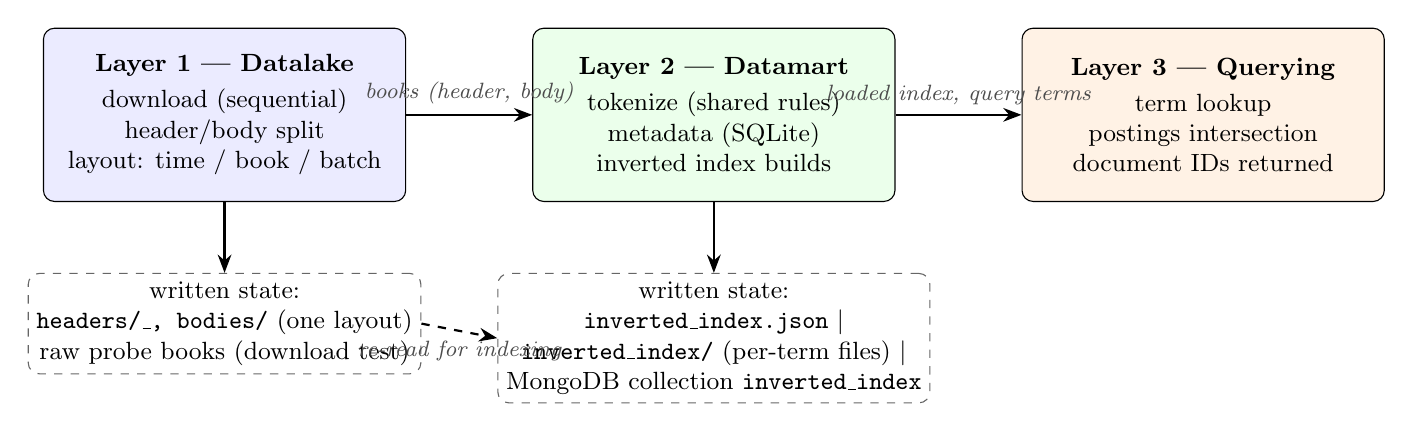
\begin{tikzpicture}[
        font=\small,
        layer/.style={draw, rounded corners, align=center, minimum height=2.2cm},
        state/.style={draw=black!60, dashed, rounded corners, align=center, inner sep=3pt},
        flow/.style={-{Stealth}, thick},
        label/.style={font=\footnotesize\itshape, text=black!70},
    ]
        % Layer 1: ingestion
        \node[layer, fill=blue!8, minimum width=4.6cm] (lake) {
            \textbf{Layer 1 --- Datalake}\\[2pt]
            download (sequential)\\
            header/body split\\
            layout: time / book / batch
        };
        % Layer 2: datamart
        \node[layer, fill=green!8, minimum width=4.6cm, right=1.6cm of lake] (mart) {
            \textbf{Layer 2 --- Datamart}\\[2pt]
            tokenize (shared rules)\\
            metadata (SQLite)\\
            inverted index builds
        };
        % Layer 3: serving
        \node[layer, fill=orange!10, minimum width=4.6cm, right=1.6cm of mart] (serve) {
            \textbf{Layer 3 --- Querying}\\[2pt]
            term lookup\\
            postings intersection\\
            document IDs returned
        };
        % Durable state
        \node[state, below=0.9cm of lake] (lakestate) {
            written state:\\
            \texttt{headers/\_, bodies/} (one layout)\\
            raw probe books (download test)
        };
        \node[state, below=0.9cm of mart] (martstate) {
            written state:\\
            \texttt{inverted\_index.json} $\mid$\\
            \texttt{inverted\_index/} (per-term files) $\mid$\\
            MongoDB collection \texttt{inverted\_index}
        };
        % Flows
        \draw[flow] (lake) -- node[label, above]{books (header, body)} (mart);
        \draw[flow] (mart) -- node[label, above]{loaded index, query terms} (serve);
        \draw[flow] (lake) -- (lakestate);
        \draw[flow] (mart) -- (martstate);
        \draw[flow, dashed] (lakestate.east) -- node[label, below]{re-read for indexing} (martstate.west);
    \end{tikzpicture}
    \caption{Stage 1 pipeline: three layers, the data that moves between them,
    and the durable state each layer writes. Downloads are sequential (one
    connection at a time); indexing reads the datalake from disk; querying
    only reads an already-built index.}
    \label{fig:pipeline}
\end{figure}

\paragraph{Layer 1 --- Datalake.}
For each book ID the engine downloads the raw Gutenberg text (or reads it
from the local corpus when offline), splits it at the official
\texttt{*** START/END OF THE PROJECT GUTENBERG EBOOK} markers, and stores the
licence header and the body as two files under one of three layouts:
\emph{time-based} (\texttt{year/month/day}), \emph{book-based}
(\texttt{book\_id/}), or \emph{batch/range-based}
(\texttt{batch\_start-batch\_end/}). The layout is a directory-structure
decision only; the stored bytes are identical.

\paragraph{Layer 2 --- Datamart.}
Bodies are tokenized with the shared rules of \cref{sec:design} and fed to
the inverted-index builders. Three structures are supported: a single JSON
file, a folder of per-term files, and a MongoDB collection. Metadata
(Title, Author, Language, paths) is extracted from the headers and persisted
in SQLite; the index builders read the corpus \emph{through} those metadata
records, which is the same path the production pipeline uses.

\paragraph{Layer 3 --- Querying.}
A query is a list of terms; a document matches when it contains \emph{every}
term. Each structure answers a term lookup with its postings list, and the
caller intersects those lists. This layer is exercised by the benchmark
workload; a user-facing search interface belongs to Stage 2 (see
\cref{sec:comment-matrix}, comments 32--33).

\paragraph{Synchronous by construction.}
The pipeline runs in one process, one book at a time: download, split, write,
tokenize, index. No step overlaps another, so every timed region in
\cref{sec:methodology} has an unambiguous start and stop. The only
concurrency anywhere in the measurement is the background thread that samples
the resident set size (\cref{tab:metrics}), and the MongoDB server process,
whose resources are explicitly excluded from client measurements
(\cref{sec:index-memory}).

\section{Design Decisions}
\label{sec:design}

\subsection{Text normalisation (shared contract)}
\label{sec:normalisation}

All four implementations apply the same normalisation, in the same order, to
every body:

\begin{enumerate}
    \item lowercase the text;
    \item drop accents/diacritics (Unicode NFD decomposition, combining marks
    removed) --- \texttt{café} $\rightarrow$ \texttt{cafe};
    \item split on any run of non-alphanumeric characters, so punctuation and
    whitespace are separators;
    \item drop tokens that contain a digit (\texttt{chapter3} is discarded);
    \item drop a small stop-word list and tokens shorter than a minimum
    length, and keep the remaining tokens in document order.
\end{enumerate}

A term's postings list is the sorted list of IDs of the documents that
contain it. Serialised, one line of the canonical form is
\texttt{postings\textbackslash ttime\textbackslash t11\textbackslash t84\textbackslash t1342}:
the term \texttt{time} appears in books 11, 84 and 1342.

\subsection{Metadata contract}
\label{sec:metadata-contract}

Headers are parsed with the same rules in the Python pipeline: fields
\texttt{Title:}, \texttt{Author:} and \texttt{Language:} are read from the
Gutenberg header; the language name is mirrored to its ISO~639 code through a
shared table (\texttt{English} $\rightarrow$ \texttt{en}); multiple authors
are split on commas, \texttt{and} and semicolons. The extracted records drive
the SQLite metadata store that the index builders read
(\cref{fig:pipeline}), so indexing goes through the same metadata contract
the production pipeline uses.

The ports mirror the parts of the contract they need: all four split header
and body at the same Gutenberg markers (the Go splitter test pins the same
fixtures as the Python one), and all four apply the identical tokenisation
and postings rules --- which is exactly what the equivalence gate verifies
per language (\cref{sec:equivalence-languages}). Metadata-field extraction
into SQLite is exercised by the Python baseline; the ports consume the
resulting bodies, so the contract they must share is the token/postings one,
and it is byte-verified.

\subsection{Storage choices under evaluation}
\label{sec:storage-choices}

\paragraph{Datalake layouts.}
Time-based layouts favour append-heavy ingestion along a timeline;
book-based layouts favour per-book lookup; batch layouts favour bulk
operations over ID ranges. All three store the same bytes, so the benchmark
can attribute every difference to directory structure alone
(\cref{sec:datalake}).

\paragraph{Index structures.}
The JSON index is a single serialised dictionary (simple, one file, whole
file must be parsed to answer any query). The folder index stores one file
per term (small reads, but one file handle per lookup). MongoDB stores one
document per term with the postings array (server-backed, queried over a
connection). None of these is declared ``best'' a priori: builds, queries,
incremental updates and on-disk footprint are measured for each
(\cref{sec:index}).

\paragraph{Language ports.}
Each port uses its ecosystem's idiomatic tools (for example
\texttt{serde}/\texttt{std::fs} in Rust, \texttt{encoding/json} and
\texttt{os} in Go, \texttt{jakarta.json} plus the driver in Java,
\texttt{json}/\texttt{pathlib}/\texttt{pymongo} in Python). The
\emph{algorithms} are held constant: the same tokenizer semantics, the same
postings construction, the same intersection query, the same synchronous
single-threaded driver. Where a runtime differs by nature (a JIT in Java),
the protocol compensates explicitly (\cref{sec:warmup}); where it cannot
compensate, the difference is reported as a limitation
(\cref{sec:limitations}).

\section{Measurement Methodology}
\label{sec:methodology}

Every number in this report was produced by one command
(\texttt{scripts/run\_tournament.sh}, \cref{sec:reproducibility}) on one
host, in one continuous run, after the equivalence gate passed. This section
documents the host, the runtimes, the metrics, the workload, and the timing
boundaries, so that each figure can be traced to a script, a configuration
and a revision.

\subsection{Host and runtimes}
\label{sec:host}

\begin{table}[htbp]
    \centering
    \caption{Host and runtime versions of the run that produced the committed
    snapshot. The full record, including the filesystem and the MongoDB
    build, is \texttt{benchmarks\_results/environment.txt}.}
    \label{tab:host}
    \begin{tabular}{@{}ll@{}}
        \toprule
        Component & Value \\
        \midrule
        CPU & Intel Core i7-10750H @ 2.60 GHz, 12 logical cores \\
        RAM & 8 GB \\
        OS / kernel & WSL2 (Ubuntu userland), Linux 6.18.33.2-microsoft-standard-WSL2 \\
        Python & 3.14.4 (+ \texttt{psutil} for RSS/CPU) \\
        Go & 1.27.2 (\texttt{linux/amd64}) \\
        Rust & 1.99.0 (\texttt{rustc}/\texttt{cargo}, stable) \\
        Java (harness) & OpenJDK 17.0.20.1, executed via \texttt{mvn exec:java} \\
        Java (JMH) & OpenJDK 21.0.12.1, shaded jar \\
        Maven & 3.9.12 \\
        MongoDB & 8.0.13, \texttt{mongod} on \texttt{localhost:27017} \\
        \bottomrule
    \end{tabular}
\end{table}

All implementations run single-threaded and synchronous
(\cref{sec:architecture}); no benchmark phase uses worker pools, async I/O or
parallel iterators. The only other process involved is \texttt{mongod}, a
separate server whose CPU and memory are \emph{not} part of the client
measurements (\cref{sec:index-memory}).

\subsection{Metric definitions}
\label{tab:metrics}

\begin{table}[htbp]
    \centering
    \caption{What each column of the result CSVs means. Identical in all four
    languages; the harness enforces the schema
    (\texttt{scripts/verify\_format.py}).}
    \label{tab:metrics}
    \begin{tabularx}{\textwidth}{@{}lX@{}}
        \toprule
        Column & Definition \\
        \midrule
        \texttt{elapsed\_seconds} & wall-clock time of one operation, from a
        monotonic clock (\texttt{time.perf\_counter}, \texttt{time.Now},
        \texttt{Instant::now}, \texttt{System.nanoTime}); per-repetition
        builds report the arithmetic mean. \\
        \texttt{stdev\_seconds} & sample standard deviation of the per-operation
        elapsed times across repetitions (query latency: across all samples). \\
        \texttt{repetitions} / \texttt{iterations} & number of timed samples
        behind the row. \\
        \texttt{memory\_mb} & \textbf{RSS delta}: resident set size of the
        benchmark process \emph{after} minus \emph{before} the operation, in
        MB, read from \texttt{/proc/self/status} (Go/Rust/Java) or
        \texttt{psutil} (Python). It measures growth caused by the operation,
        not the total footprint of the process. \\
        \texttt{peak\_rss\_mb} & largest resident set size of the benchmark
        process observed while the operation ran, sampled every
        \fixed{50} ms by a background thread plus one final sample; across
        repetitions the maximum is reported. \\
        \texttt{cpu\_percent} & process CPU time (user + system) divided by
        wall-clock time, $\times 100$; above 100 means more than one core was
        saturated. \\
        \bottomrule
    \end{tabularx}
\end{table}

Both memory series describe the \emph{benchmark client process only}. For the
MongoDB structure, the server's own memory and disk are reported separately
(\cref{sec:index-memory}); they are never folded into the client's RSS.

\subsection{Corpus and workload}
\label{sec:workload}

\begin{table}[htbp]
    \centering
    \caption{Workload actually executed by every language.}
    \label{tab:workload}
    \begin{tabularx}{\textwidth}{@{}lX@{}}
        \toprule
        Parameter & Value \\
        \midrule
        Corpus & \fixed{100} Project Gutenberg books, tracked in
        \texttt{data\_source/} (bodies $\approx$\fixed{59} MB, headers
        $\approx$0.4 MB); book IDs listed in
        \texttt{benchmarks\_results/equivalence\_report.json}. \\
        Query workload & \fixed{30} active queries from the shared file
        \texttt{src/utils/benchmarks/queries.txt} (one query per line,
        terms separated by a single space; comments start with \texttt{\#}).
        Semantics: a document matches when it contains every term; an unknown
        term yields an empty result. \\
        Query samples & \fixed{5} repetitions $\times$ \fixed{30} queries =
        \fixed{150} timed samples per structure per language. \\
        Datalake lookup & \fixed{100} books located once per layout (header
        and body read). \\
        Download probe & \fixed{10} books downloaded sequentially over one
        connection; no concurrency anywhere in the pipeline. \\
        Build batches & \fixed{25, 50, 250, 500, 1000, 5000, 10000} books;
        5 repetitions up to 1000, 3 for 5000, 2 for 10000. \\
        Update batches & base indexes of \fixed{25, 50, 250, 500, 1000}
        books, each extended with \fixed{5} new books, \fixed{5}
        repetitions per base size (\cref{sec:index-updates}). \\
        Recovery & interrupt after \fixed{50} of \fixed{100} books, then
        resume; report processed, duplicated and lost IDs plus detection and
        processing time. \\
        \bottomrule
    \end{tabularx}
\end{table}

The scalability builds reuse the corpus by repetition: a ``10{,}000-book
batch'' is the \fixed{100}-book corpus indexed repeatedly until the batch
size is reached, so batch size measures index size, not corpus diversity.
The update experiment is the exception: it uses fresh synthetic book IDs
(\texttt{base\_size}$\times$100 + offset), so added books are genuinely new
terms and never collide with the base.

\subsection{Warm-up}
\label{sec:warmup}

Only the Java harness warms up, because Java is the only runtime with a JIT
compiler: before timing, each Java structure performs one unmeasured build of
the smallest batch and discards its artifacts, so the measured builds run on
already-compiled code. Python, Go and Rust are measured exactly as they
start: no warm-up, no discarded round. JMH numbers
(\cref{sec:jmh}) use JMH's own warm-up iterations and are reported
separately; they are never mixed with the cross-language figures.

\subsection{Cache, disk and network state}
\label{sec:environment-state}

\begin{itemize}
    \item \textbf{Artifact directories.} Every timed phase starts from a
    freshly cleaned artifact tree: the previous run's datalake, index and
    result files are deleted before the phase begins, so no phase reads a
    cache written by another.
    \item \textbf{OS page cache.} The tournament does not drop the system
    page cache (that requires root and would perturb the host). Files read
    twice within one phase may therefore be served from RAM. This affects all
    languages equally within a phase and is listed as a limitation
    (\cref{sec:limitations}).
    \item \textbf{Disk.} All artifacts live on the same filesystem as the
    repository (WSL2 / NTFS-backed). \texttt{disk\_usage.csv} reports file
    counts, directory counts and bytes for each layout and each index
    structure after storing the same corpus.
    \item \textbf{Network.} Only the download probe touches the network: ten
    sequential GETs, one connection at a time, measured with the same clock
    as everything else. Every other phase is fully offline and reads the
    tracked corpus from disk.
\end{itemize}

\subsection{Timing boundaries}
\label{sec:timing-boundaries}

\begin{itemize}
    \item \textbf{Write throughput} times the storage call itself: split
    header+body written to the layout (the download is timed separately), one
    book per iteration, \fixed{100} iterations per layout.
    \item \textbf{Download throughput} starts before the HTTP request and
    stops after the response body is fully read and written to disk.
    \item \textbf{Lookup} starts before locating the book's files under the
    layout and stops after both files are read into memory.
    \item \textbf{Index build} starts before the first token is produced and
    stops after the structure is fully written (JSON flushed, per-term files
    closed, or MongoDB insert acknowledged).
    \item \textbf{Query} starts before the postings lookup of the first term
    and stops after the intersection of all terms is computed.
    \item \textbf{Incremental update} starts before the first of the five new
    books is tokenized and stops after the structure is durably updated.
\end{itemize}

\subsection{Repetition and uncertainty}
\label{sec:uncertainty}

Each timed operation is repeated as specified in \cref{tab:workload}; plots
show the mean and, where a deviation band appears, it is the sample standard
deviation across those repetitions (\texttt{stdev\_seconds}). Readers can
assess uncertainty from the raw \texttt{repetitions} and \texttt{stdev}
columns committed next to every chart. No result is discarded, no outlier is
trimmed, and no phase is run twice to pick the better run: the committed
snapshot is a single continuous tournament.

\subsection{Coverage: what was compared with what}
\label{sec:coverage}

\begin{table}[htbp]
    \centering
    \caption{Language $\times$ structure coverage of the timed workload
    (D=datalake layouts, J=JSON index, F=folder index, M=MongoDB index,
    S=SQLite metadata).}
    \label{tab:coverage}
    \begin{tabular}{@{}lcccc@{}}
        \toprule
        Language & Datalake & JSON & Folder & MongoDB \\
        \midrule
        Python & D, S & J, F, M & & \\
        Go & D, S & J, F, M & & \\
        Rust & D, S & J, F, M & & \\
        Java & D, S & J, F, M & & \\
        \bottomrule
    \end{tabular}
\end{table}

Every language runs the full matrix: three datalake layouts plus the three
index structures, with identical parameters. MongoDB is skipped consistently
and identically by all four ports when the server is unreachable, so no
figure silently compares a MongoDB-less run with a MongoDB run.

\subsection{Revisions and provenance}
\label{sec:provenance}

Each chart in this report maps to (i) the script that produced it, (ii) the
raw CSVs in \texttt{benchmarks\_results/}, (iii) the configuration constants
listed in \cref{tab:workload}, and (iv) the Git revision recorded in
\texttt{benchmarks\_results/environment.txt} at run time. The mapping is
tabulated in \cref{sec:reproducibility}.

\section{Cross-Language and Cross-Structure Equivalence}
\label{sec:equivalence}

Speed differences are only meaningful if the implementations compute the same
thing. Two equivalence gates run before any timing is reported, and both
commit their evidence next to the results.

\subsection{Gate 1: the four languages agree}
\label{sec:equivalence-languages}

The checker (\texttt{src/utils/benchmarks/equivalence\_check.py}) selects
\fixed{100} books from the corpus, evenly spaced by ID, and runs every
port's \texttt{equivalence} mode over them. Each port writes one canonical
file with three sections:

\begin{enumerate}
    \item \texttt{tokens} --- the token stream of every sample book
    (\texttt{tokens<TAB>book\_id<TAB>token...});
    \item \texttt{postings} --- the inverted index built from those tokens
    (\texttt{postings<TAB>term<TAB>id...});
    \item \texttt{query} --- the answer to every one of the \fixed{30}
    shared queries (\texttt{query<TAB>ordinal<TAB>id...}).
\end{enumerate}

The four files are compared byte for byte. The run recorded in
\texttt{benchmarks\_results/equivalence\_report.json} produced the same
SHA-256 digest in all four languages,

\begin{center}
    \texttt{cdaa9369cbd91c4f89550efdcdd7c5c21e61adc97bd49f6e415b8e57d65ce2e4},
\end{center}

with \texttt{all\_equal: true}. Identical bytes imply identical tokens,
identical postings and identical query answers: the cross-language latency
comparison in \cref{sec:language-performance} compares the same work
everywhere. The tournament refuses to run any timed phase if this gate fails.

\subsection{Gate 2: the three structures agree}
\label{sec:equivalence-structures}

Within a language, the latency chart compares three index structures. The
test \texttt{tests/test\_datamarts/test\_structure\_equivalence.py} builds
the same corpus into the JSON file, the folder index and MongoDB, then
queries \emph{every} term of the corpus plus absent terms on each structure
and asserts that all answers are identical. A second case repeats the check
\emph{after} adding the same new book to each structure through its own
incremental-update path, so an update cannot make one structure diverge
silently. All cases pass (\cref{tab:equivalence-tests}); the MongoDB cases
skip themselves with an explicit reason when the server is down, and the
tournament only runs timed MongoDB phases when the server is reachable.

\begin{table}[htbp]
    \centering
    \caption{Cross-structure equivalence cases and results.}
    \label{tab:equivalence-tests}
    \begin{tabular}{@{}llc@{}}
        \toprule
        Case & Structures compared & Result \\
        \midrule
        All terms + absent terms, fresh build & JSON = folder & identical \\
        All terms + absent terms, fresh build & JSON = folder = MongoDB & identical \\
        Re-queried after the same incremental update & JSON = folder = MongoDB & identical \\
        \bottomrule
    \end{tabular}
\end{table}

\subsection{What equivalence does and does not prove}
\label{sec:equivalence-scope}

The gates prove \emph{functional} equivalence on this corpus and workload:
same tokens, same postings, same answers. They say nothing about speed ---
that is exactly what the following sections measure. Conversely, the
latency charts inherit the gates' guarantee: every bar in them comes from an
implementation that is known to answer identically.

\section{Language Performance Trade-offs}
\label{sec:language-performance}

This section compares the four \emph{implementations} on the shared workload.
It reports what was measured; it does not generalise to the languages
themselves (see \cref{sec:limitations}).

\subsection{Executive radar}
\label{sec:radar}

\begin{figure}[htbp]
    \centering
    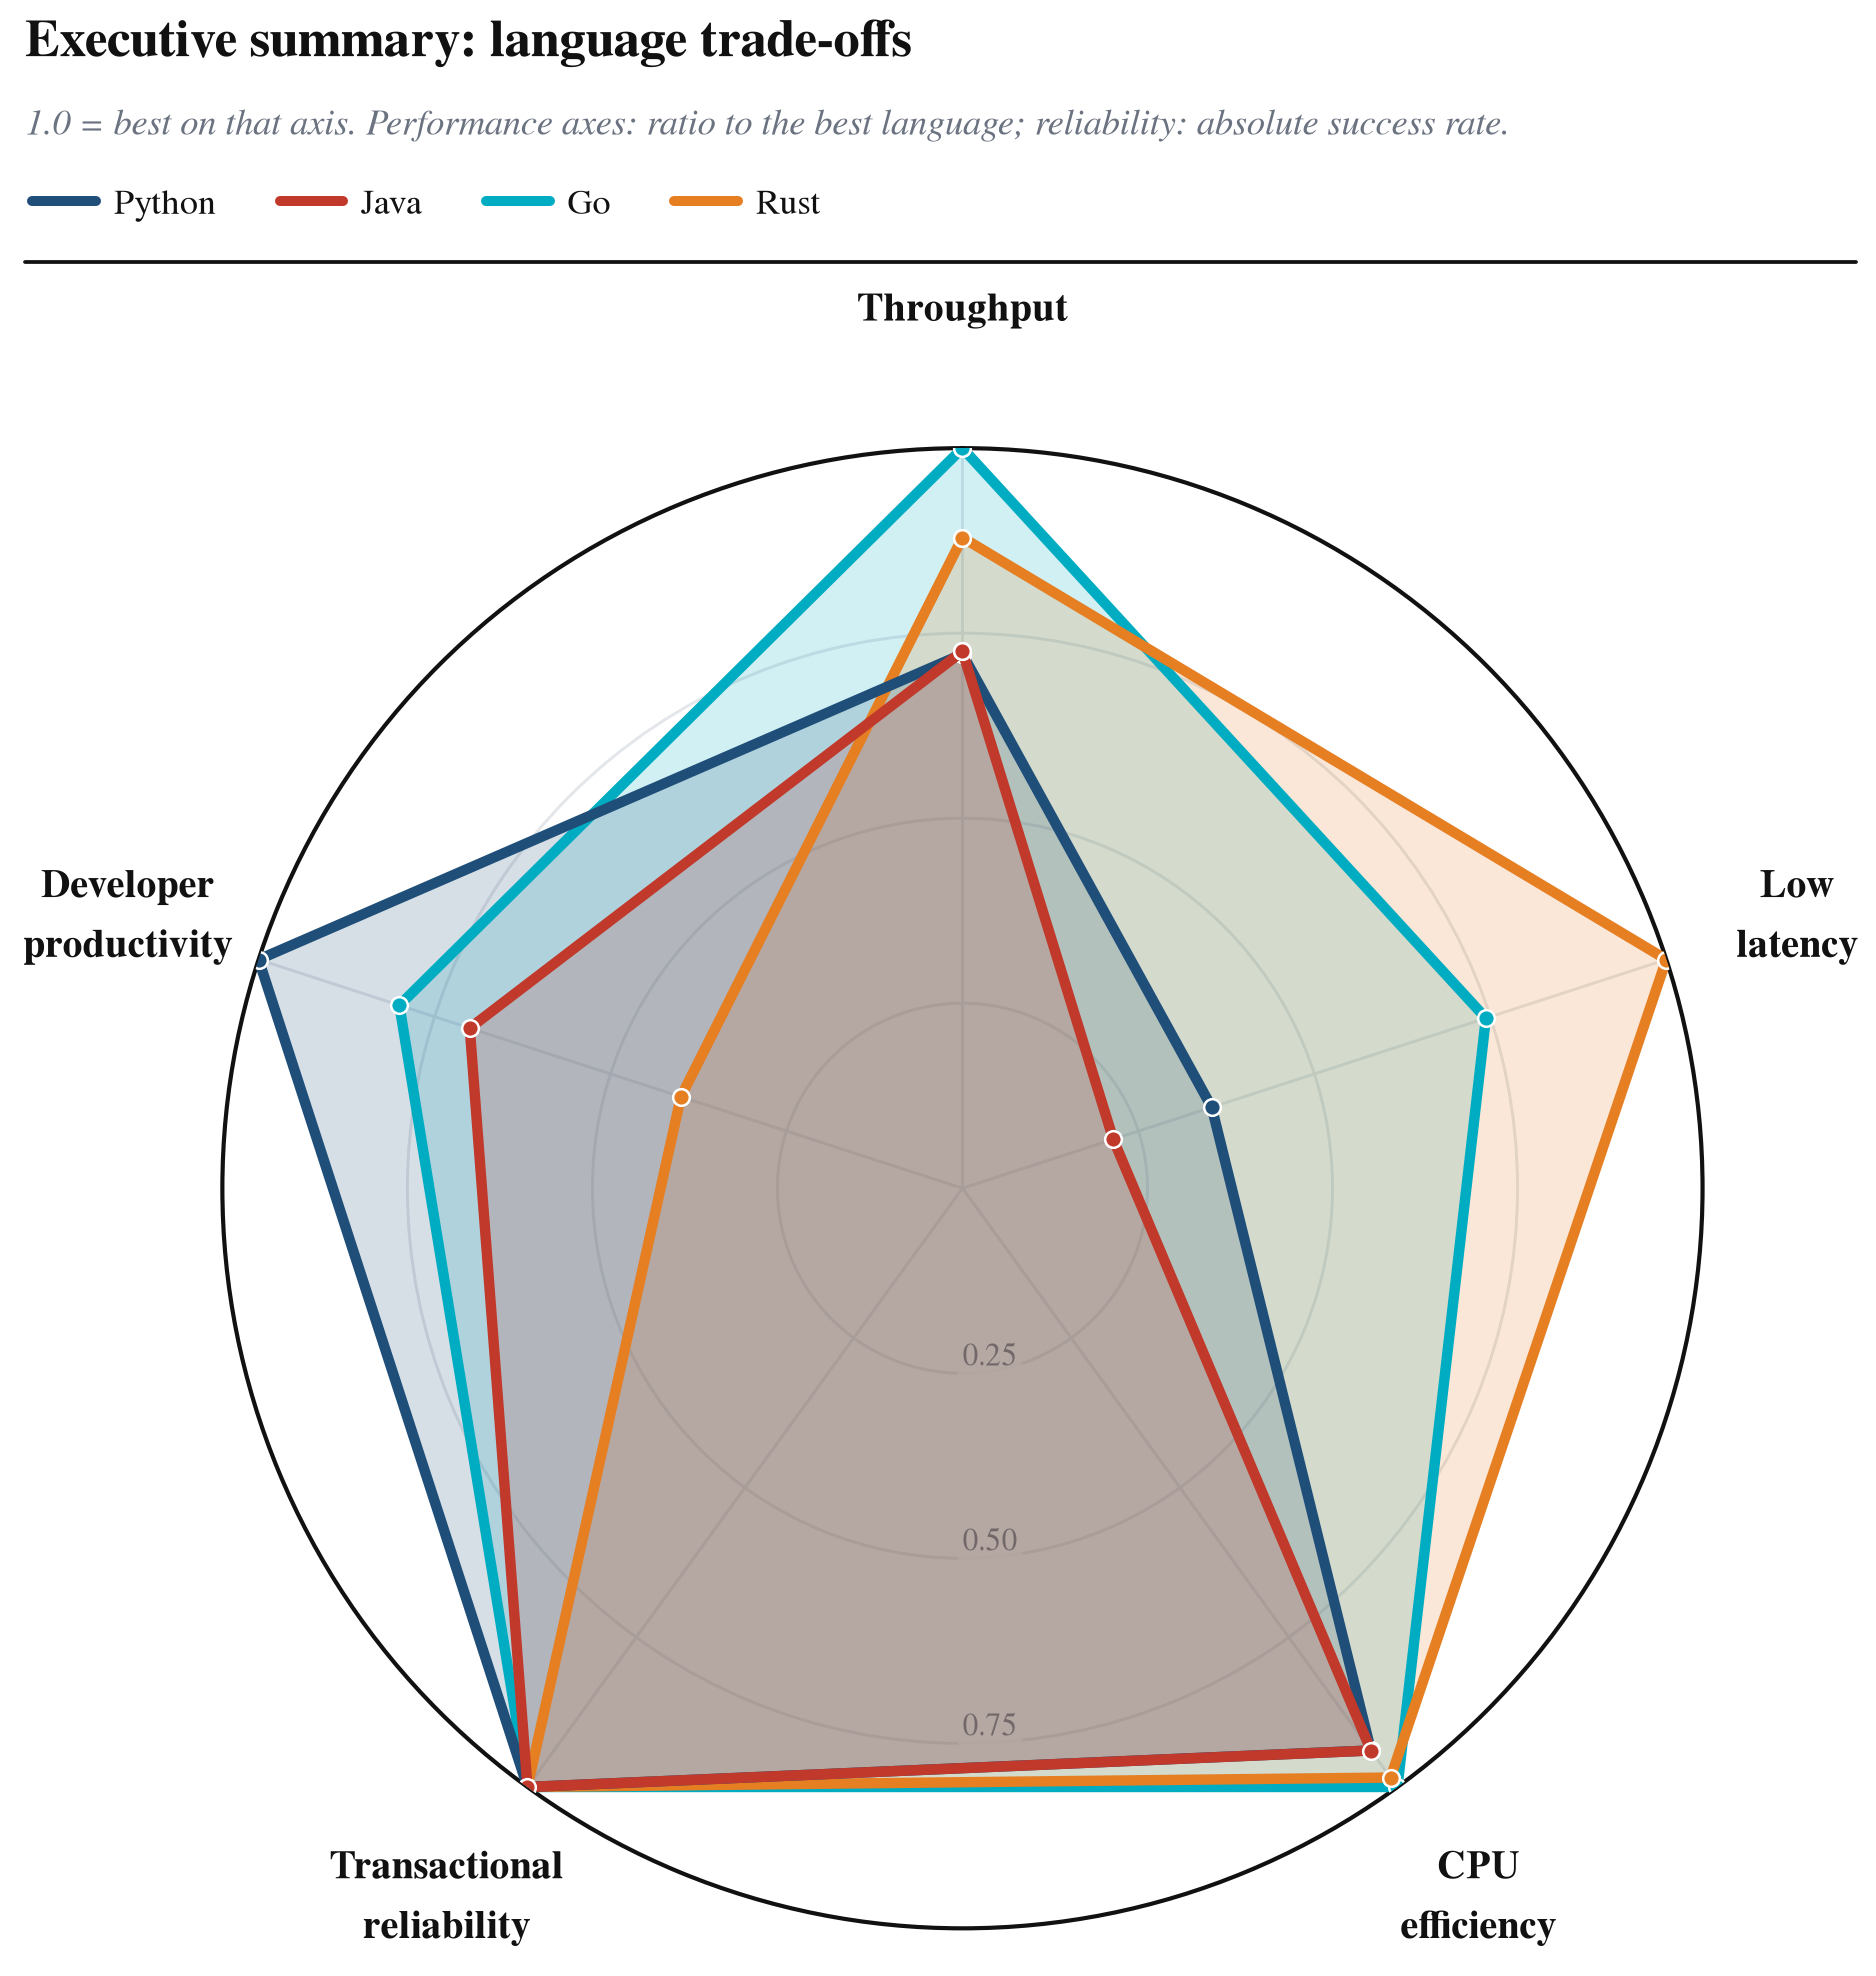
\includegraphics[width=0.60\textwidth]{radar/executive_radar.png}
    \caption{Five-axis executive summary (generated by
    \texttt{src/visualizations/main.py} from
    \texttt{benchmarks\_results/}). Throughput, low latency and CPU
    utilisation are ratios to the best implementation on tests run by all
    four languages; reliability is an absolute rate; ``developer
    productivity'' is a \textbf{qualitative} team score, although the axis
    label in the image does not yet say so (\cref{sec:radar}).}
    \label{fig:radar}
\end{figure}

The radar of \cref{fig:radar} summarises five axes. Four are computed from
the CSVs:

\begin{itemize}
    \item \textbf{Throughput, low latency, CPU efficiency} --- ratios to the
    best measured implementation on tests run by \emph{all four} languages,
    so no axis is biased by a partial run;
    \item \textbf{Transactional reliability} --- an absolute success rate,
    $1 - (\text{lost} + \text{duplicated}) / \text{total books}$, averaged
    over the recovery scenarios. It is deliberately \emph{not} rescaled to
    the best language: an implementation that loses books must never be
    stretched to 1.0.
\end{itemize}

The fifth axis, \textbf{developer productivity}, is a \emph{qualitative
score} assigned by the team (Python 1.0, Go 0.8, Java 0.7, Rust 0.4) from
the effort observed while porting the pipeline: lines of boilerplate,
error-handling ceremony, iteration speed and tooling friction. It is not
measured by any benchmark and no conclusion in \cref{sec:conclusions} rests
on it; this paragraph is the authoritative reading of that axis, whose
rendered label does not yet say ``qualitative'' (\cref{sec:future}).
Memory is intentionally absent from the radar: RSS deltas are too
noisy to summarise in one number; they are shown in full in
\cref{fig:scalability-memory}.

\paragraph{Scores in the current snapshot.}
Throughput: Go 1.00, Rust 0.88, Java 0.73, Python 0.72. Low latency: Rust
1.00, Go 0.74, Python 0.35, Java 0.21. CPU axis: Go 1.00, Rust 0.98, Java
0.94, Python 0.94. Reliability: 1.00 for all four. Three caveats bound this
summary:

\begin{itemize}
    \item The throughput axis is the geometric mean of the three datalake
    write rates and the download rate. The rendered figure takes only the
    fifth of the five download rounds instead of their mean (the per-round
    rows are in \texttt{throughput.csv}). With the five-round mean the scores
    are Go 1.00, Rust 0.82, Python 0.68 and Java 0.68: Go and Rust keep their
    order, Python and Java become indistinguishable.
    \item The CPU axis scores \emph{lower} mean CPU utilisation during the
    index builds as better, so a client that waits on \texttt{mongod} scores
    well. It measures utilisation, not efficiency; with every harness pinned
    to one core the four raw values span only 85.4--90.9\%, and no conclusion
    is drawn from it.
    \item The reliability axis is 1.0 by construction of the resume check
    (\cref{sec:datalake-recovery}) and cannot discriminate between the
    implementations.
\end{itemize}

\subsection{Throughput and latency overview}
\label{sec:throughput-latency}

\begin{figure}[htbp]
    \centering
    \begin{minipage}[t]{0.48\textwidth}
        \centering
        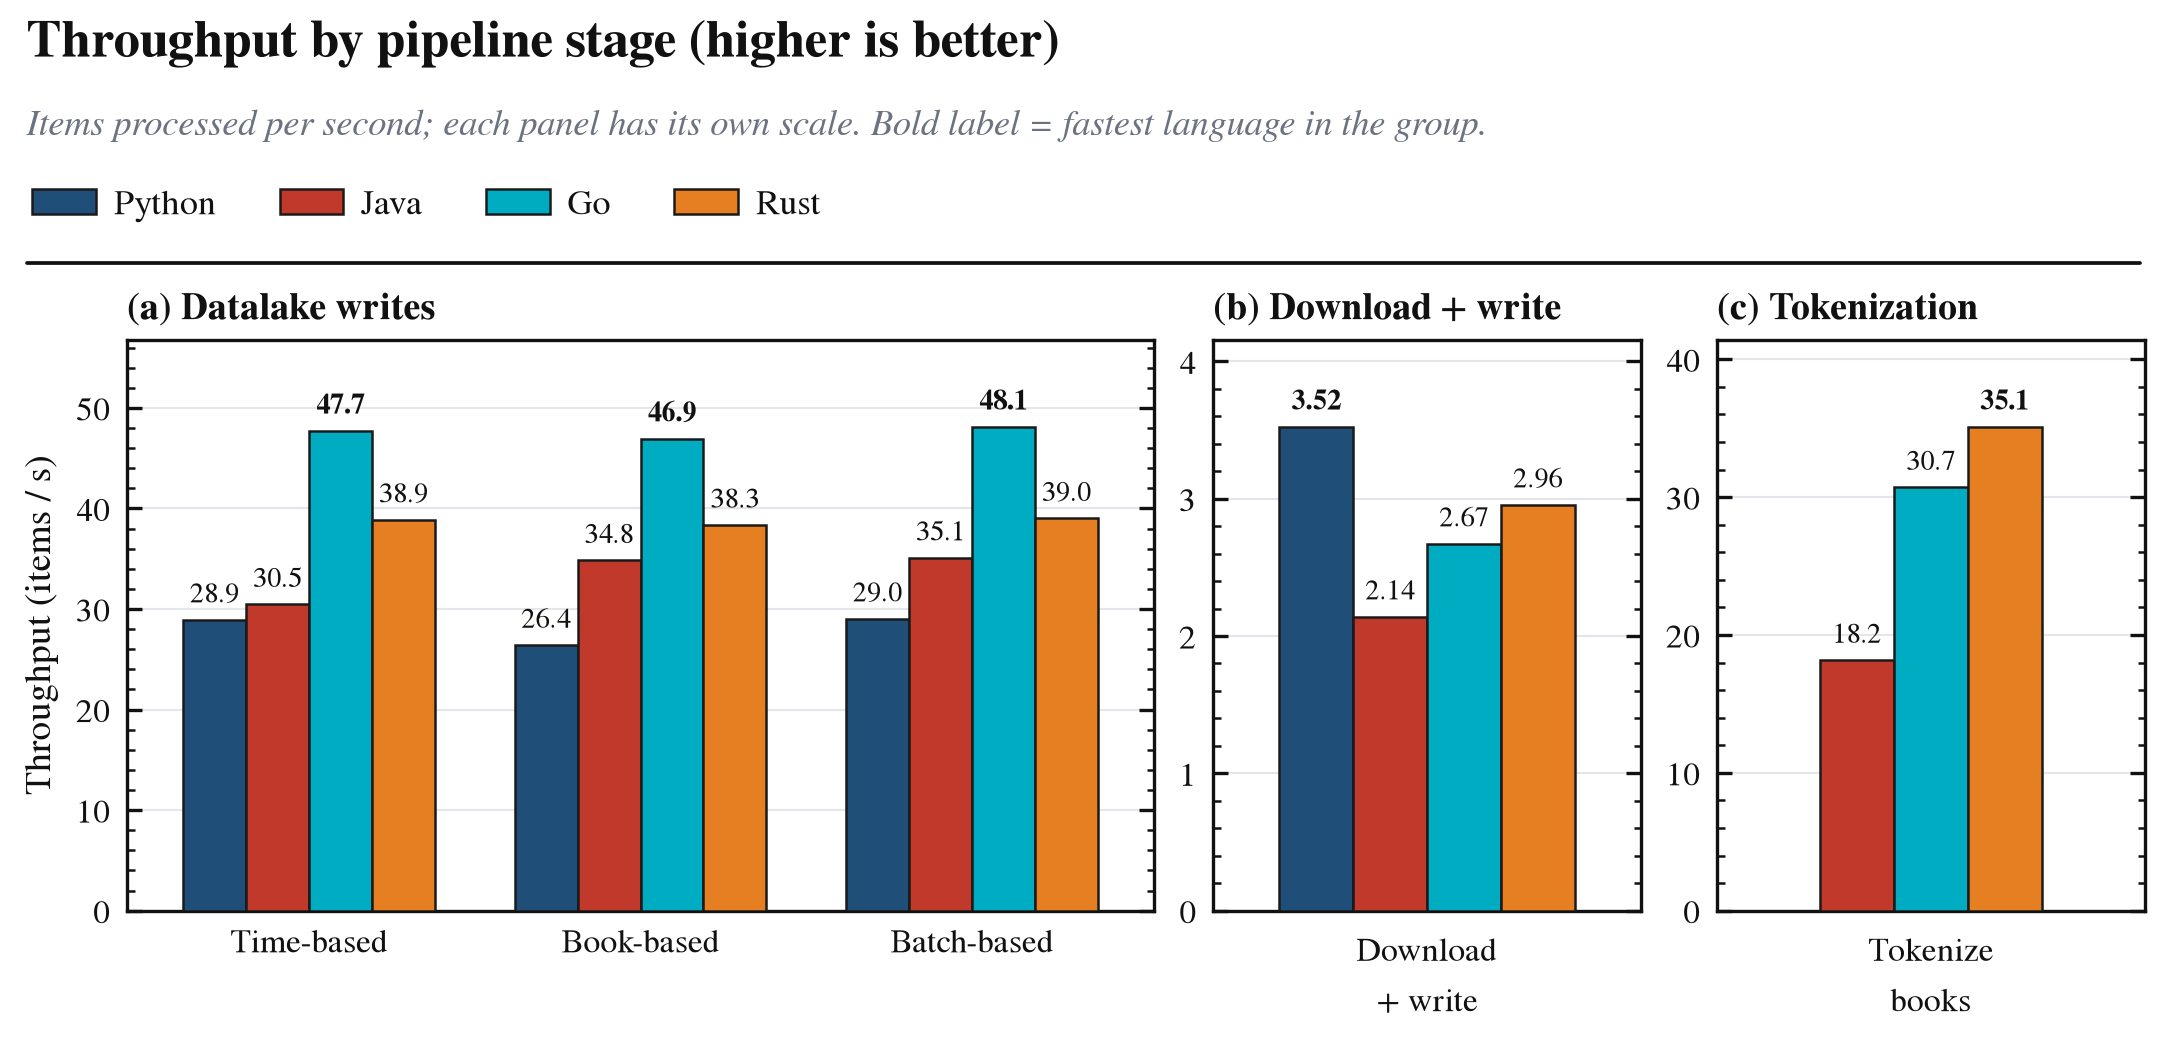
\includegraphics[width=0.95\textwidth]{throughput/throughput.png}
        \caption{Throughput per pipeline stage: (a) datalake writes, one
        timed run of 100 books per layout; (b) download + write, 10 books
        per round, showing the fifth of five rounds (five-round means in
        \cref{tab:download}); (c) tokenisation of the corpus (not recorded
        by the Python harness).}
        \label{fig:throughput}
    \end{minipage}\hfill
    \begin{minipage}[t]{0.48\textwidth}
        \centering
        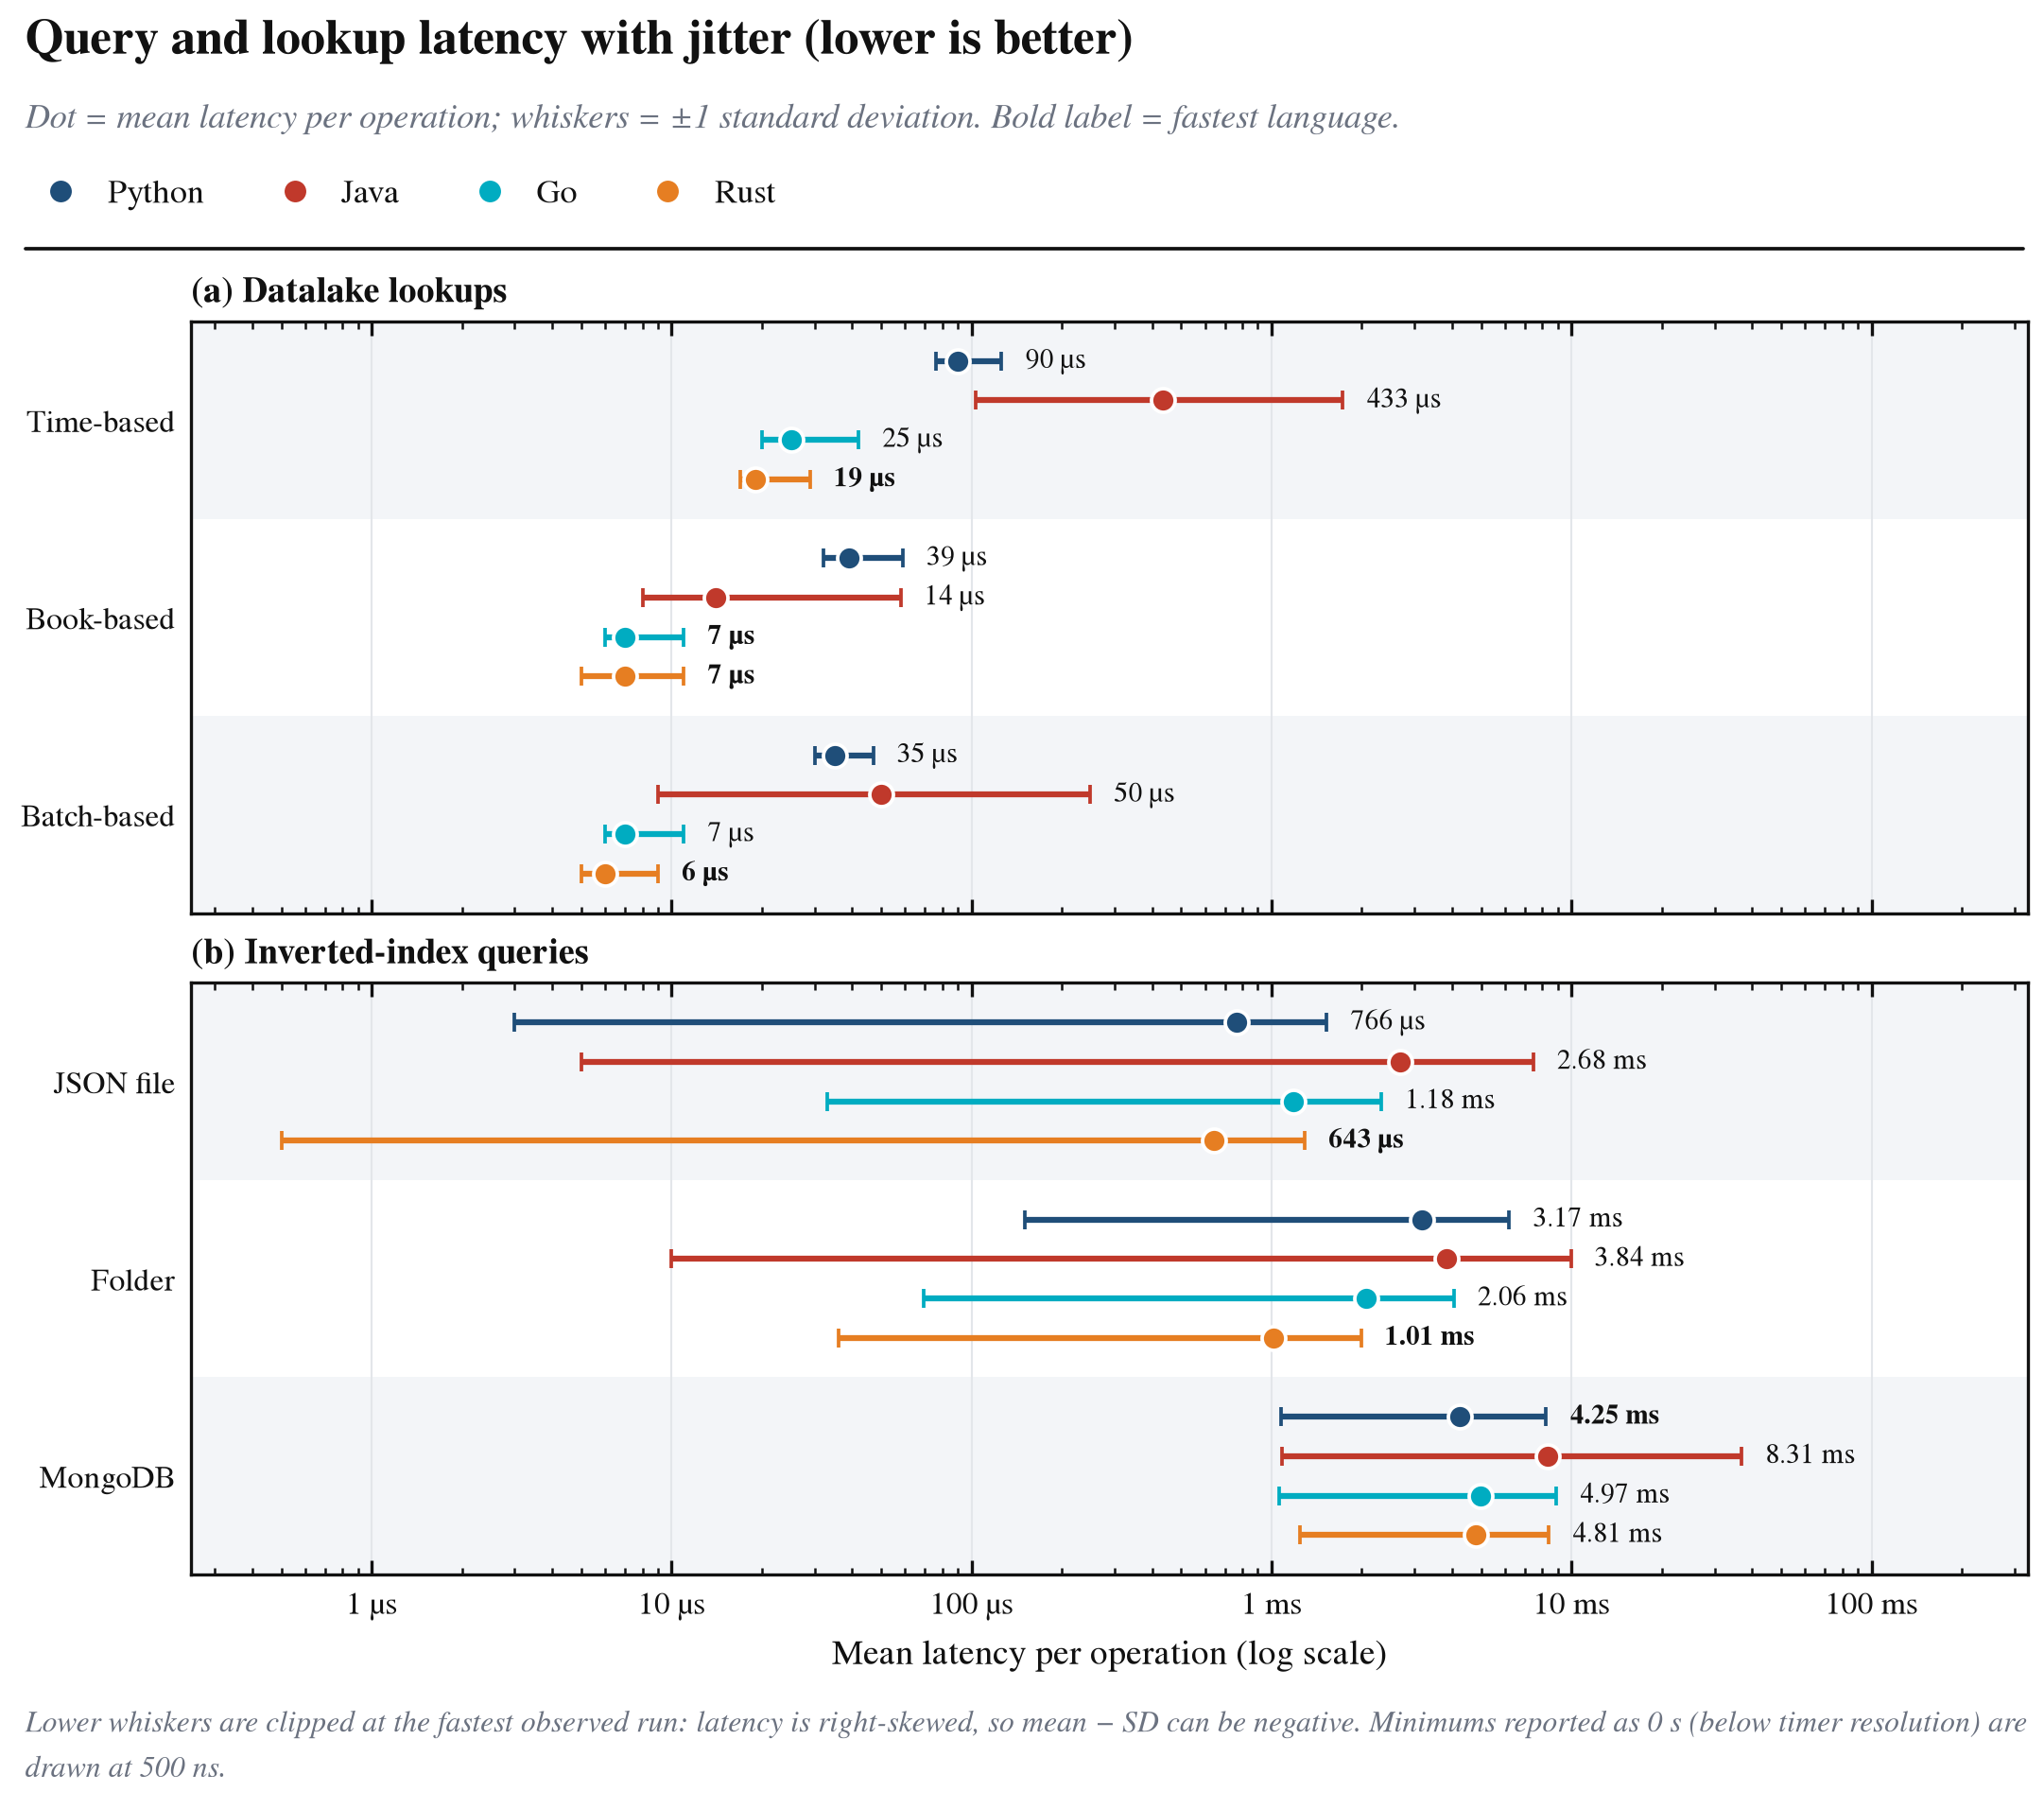
\includegraphics[width=0.95\textwidth]{latency/latency.png}
        \caption{Lookup latency per datalake layout (100 samples) and query
        latency per index structure (150 samples on the 10{,}000-book
        index). Dot = mean; whiskers = $\pm 1$ SD, clipped at the
        minimum.}
        \label{fig:latency}
    \end{minipage}
\end{figure}

\Cref{fig:throughput,fig:latency} show the two extremes of the workload.
They come from the same tournament run, so their relative ordering is
meaningful; the absolute values are specific to the host of
\cref{tab:host}, and the raw rows sit next to them in
\texttt{benchmarks\_\allowbreak results/}.

The reading rule for this whole report: differences between the four
implementations describe \emph{these implementations, on this corpus, under
this protocol}. Where an explanation requires a language-level cause (JIT
behaviour, allocator strategy, runtime overhead), it is stated as a
hypothesis and flagged as such, not as a measured fact.

\subsection{Effect of the corrective changes}
\label{sec:refactor-effect}

Between the snapshot discussed in the previous version of this report
(results commit \texttt{28d4c3f}, run of 25 October, code \texttt{b104a9a})
and the current one (results commit \texttt{9e53348}, run of 28 October,
code \texttt{0482a5e}), five changes were made to the ports and the harness.
None of them alters what is computed (the equivalence digest of
\cref{sec:equivalence} is unchanged) or introduces concurrency.
\Cref{tab:refactor-effect} pairs each change with the metric it should
move.

\begin{table}[htbp]
    \centering
    \small
    \caption{Previous $\to$ current value of the metrics each corrective
    change targets (one tournament run per snapshot; raw rows in
    \texttt{benchmarks\_results/} at \texttt{28d4c3f} and \texttt{9e53348}).}
    \label{tab:refactor-effect}
    \begin{tabularx}{\textwidth}{@{}Xrrrr@{}}
        \toprule
        Metric & Python & Go & Rust & Java \\
        \midrule
        \multicolumn{5}{@{}l}{\emph{Durable writes (temporary file, fsync, rename) in every port}} \\
        Datalake write, items/s (mean of 3 layouts) & 29.2$\to$28.1 & 68.0$\to$47.6 & 79.1$\to$38.7 & 64.6$\to$33.5 \\
        \multicolumn{5}{@{}l}{\emph{Pooled HTTP connection; five interleaved download rounds}} \\
        Download + write, items/s (5-round mean) & 1.48$\to$3.24 & 3.32$\to$3.12 & 1.32$\to$2.60 & 2.87$\to$1.88 \\
        \multicolumn{5}{@{}l}{\emph{Rust MongoDB update sent as one bulk write per book}} \\
        MongoDB update, base 25, ms & 134$\to$128 & 124$\to$113 & 474$\to$122 & 130$\to$145 \\
        MongoDB update, base 1{,}000, ms & 381$\to$397 & 293$\to$299 & 643$\to$286 & 294$\to$305 \\
        \multicolumn{5}{@{}l}{\emph{Collection dropped, not emptied, before every build}} \\
        MongoDB \texttt{storageSize}, MiB & 557.1$\to$29.6 & 558.9$\to$5.4 & 324.6$\to$16.1 & 38.2$\to$13.1 \\
        \multicolumn{5}{@{}l}{\emph{Every harness pinned to one logical core}} \\
        Build, 10{,}000 books, JSON, s & 167.1$\to$170.9 & 66.0$\to$71.4 & 196.4$\to$208.1 & 947.0$\to$1154.4 \\
        Build, 10{,}000 books, folder, s & 234.7$\to$215.3 & 69.9$\to$78.4 & 202.7$\to$198.1 & 955.2$\to$1130.0 \\
        Build, 10{,}000 books, MongoDB, s & 220.7$\to$181.5 & 76.6$\to$83.8 & 206.6$\to$200.7 & 929.1$\to$1185.1 \\
        \bottomrule
    \end{tabularx}
\end{table}

\paragraph{Durability, not language, explained most of the earlier write gap.}
In the previous snapshot only the Python baseline wrote datalake files
through a temporary file, \texttt{fsync} and rename; the ports used plain
writes, and the write-throughput spread was $3.0\times$ (27.3--82.8
items/s). With the same protocol in all four, the ports lost 30\% (Go), 51\%
(Rust) and 48\% (Java) of their rate, while Python, whose write path did not
change, moved by $-4\%$; the spread fell to $1.8\times$ (26.4--48.1
items/s). Python thus acts as an internal control: the host-level
differences between the two runs moved its unchanged write path by a few
per cent only, so the ports' drops are attributable to the added
synchronisation. Client CPU utilisation during the writes fell in every port
(Go 35--38\% $\to$ 17--18\%, Rust 17--19\% $\to$ 10--13\%, Java 36--70\% $\to$ 27--37\%), as
expected when a phase becomes storage-bound (\cref{sec:datalake-throughput}).

\paragraph{Rust's MongoDB update cost was a protocol artefact.}
The Rust port previously issued one \texttt{update\_one} round trip per
distinct term; it now sends the same upserts as one unordered bulk write,
like the other three. Its single-book update at base 25 fell from 474 to
122~ms ($3.9\times$) and now lies within the 113--145~ms band of the other
ports. The previous flat Rust curve ($1.36\times$ from base 25 to 1{,}000)
came from a large constant round-trip cost hiding the growth; with the bulk
write Rust grows $2.34\times$, in line with the others
(\cref{sec:index-updates}).

\paragraph{Collection reuse inflated the MongoDB footprint.}
Dropping the collection before each build reduced the reported
\texttt{storageSize} from 38.2--558.9~MiB to 5.4--29.6~MiB. The remaining
$5.5\times$ spread for identical logical content shows that the figure is
still not a reliable footprint measure (\cref{sec:index-structures}).

\paragraph{Pinning penalised the runtimes that parallelise their own housekeeping.}
Under the single-core budget the 10{,}000-book builds became 8--12\% slower
in Go and 18--28\% slower in Java, whereas Python and Rust, whose timed code
runs no background runtime threads, changed by $-18$ to $+6\%$ without a
consistent direction. Go's concurrent garbage collector and the JVM's
collector and JIT compiler threads previously ran on other cores and now
share the measured one; in addition, with one processor reported, HotSpot's
ergonomics select the Serial collector instead of G1, so the current Java
series runs under a different collector than the previous one. This
attribution is a hypothesis: no GC log was recorded. We do not attribute the
Python and Rust movements.

\paragraph{What the comparison cannot separate.}
Both snapshots are single runs, and more than the five changes differ
between them: the memory visible to the WSL2 virtual machine (7.66 $\to$
9.71~GiB), the toolchain patch versions (Go 1.27.1 $\to$ 1.27.2, Rust 1.99.0
$\to$ 1.99.1, OpenJDK 21.0.12.1 $\to$ 21.0.13) and the MongoDB server record
(\texttt{mongo:7} in Docker now; the previous record could not identify the
server). Only the effects with a direct mechanism (synchronisation, bulk
write, collection drop) are attributed above; the rest of this report
interprets the current snapshot on its own.

\section{Datalake Structure Evaluation}
\label{sec:datalake}

The datalake stores the same header/body pairs under three layouts. This
section evaluates them on the dimensions the assignment asks for: write and
download throughput, document lookup, discovery of new books, storage
overhead, and recovery after an interruption. All numbers come from
\texttt{datalake\_experiments.py} (Python baseline; the network probe from
\texttt{download\_probe.py}) and the equivalent
\texttt{datalake\_bench} code in each port, with the parameters of
\cref{tab:workload}.

\subsection{Write and download throughput}
\label{sec:datalake-throughput}

Write throughput is one timed run per layout that reads each of the
\fixed{100} tracked headers and bodies from \texttt{data\_source/} and stores
them through the layout's storage path. Since the current snapshot every
implementation writes each file to a temporary sibling, forces it to stable
storage with \texttt{fsync} and renames it into place
(\cref{sec:refactor-effect}). The download is a separate experiment:
\fixed{10} books fetched sequentially in each of \fixed{5} rounds through one
pooled connection per language, timed from before the HTTP request until the
body is written to disk. The rounds interleave the languages round-robin, so
no language downloads at a systematically different hour of the run. Both
experiments operate on the same \fixed{100}-book corpus.

\paragraph{Writes.}
Go stored the corpus at 46.9--48.1 items/s, Rust at 38.3--39.0, Java at
30.5--35.1 and Python at 26.4--29.0 (\cref{fig:throughput}a): 21~ms per book
for Go and 36~ms for Python, each book being two synchronised files. The
layout matters little. Within each implementation the three layouts differ
by at most 3\% in Go and Rust, 10\% in Python and 15\% in Java, and the
book-based layout, which creates one directory per book (plus, in Python, a
\texttt{metadata.json} per book), is the slowest in Python, Go and Rust.
Client CPU utilisation during the writes is 10--13\% (Rust), 17--18\% (Go)
and 27--37\% (Java): the phase is bound by storage synchronisation, not by
computation. The remaining ordering of the ports (Go, Rust, Java) is not
explained by the data collected.

\paragraph{Downloads.}
\Cref{tab:download} summarises the five rounds. The probe is network-bound
(client CPU 1.5--6.3\% in Go and Rust), so it characterises the HTTP clients
and the path to Project Gutenberg rather than computation. Python
(3.24~items/s) and Go (3.12) overlap within one standard deviation; Rust is
lower (2.60) and Java lowest (1.88). Java's mean is pulled down by a first
round of 11.2~s (0.89~items/s; median 2.13), and its client uses 25--44\% CPU;
since every round starts a fresh JVM through Maven, start-up and JIT cost is
a plausible cause, which we did not isolate. Panel~(b) of
\cref{fig:throughput} shows the fifth round only, not these means
(\cref{sec:radar}).

\begin{table}[htbp]
    \centering
    \caption{Download + write throughput, \fixed{10} books per round,
    \fixed{5} interleaved rounds per language (\texttt{throughput.csv}).
    The previous snapshot had a single round per language, taken at
    different hours and without connection pooling in Python and Rust.}
    \label{tab:download}
    \begin{tabular}{@{}lcccc@{}}
        \toprule
        Language & Mean $\pm$ SD (items/s) & Min--max & Median & Previous ($n=1$) \\
        \midrule
        Python & 3.24 $\pm$ 0.29 & 2.90--3.52 & 3.39 & 1.48 \\
        Go & 3.12 $\pm$ 0.37 & 2.67--3.47 & 3.31 & 3.32 \\
        Rust & 2.60 $\pm$ 0.25 & 2.25--2.96 & 2.64 & 1.32 \\
        Java & 1.88 $\pm$ 0.56 & 0.89--2.22 & 2.13 & 2.87 \\
        \bottomrule
    \end{tabular}
\end{table}

\subsection{Document lookup}
\label{sec:datalake-lookup}

\fixed{100} books are located once per layout: the harness resolves the
book's directory and checks that both its header and its body exist; the
files are not read. The book-based and batch-based layouts derive the
directory arithmetically from the ID, whereas the time-based layout must list
its hour directories, newest first, and probe each until it finds the book.
\Cref{tab:datalake-lookup} reports the mean and, because several series are
right-skewed, the minimum.

\begin{table}[htbp]
    \centering
    \caption{Datalake lookup latency, 100 books per layout, in $\mu$s: mean
    (minimum) per language; raw rows in
    \texttt{benchmarks\_results/<language>/statistics.csv}.}
    \label{tab:datalake-lookup}
    \begin{tabular}{@{}lcccc@{}}
        \toprule
        Layout & Python & Go & Rust & Java \\
        \midrule
        Time-based & 90 (76) & 25 (20) & 19 (17) & 433 (103) \\
        Book-based & 39 (32) & 7 (6) & 7 (5) & 14 (8) \\
        Batch-based & 35 (30) & 7 (6) & 6 (5) & 50 (9) \\
        \bottomrule
    \end{tabular}
\end{table}

The time-based layout is the slowest in every implementation (19--433~$\mu$s
mean, 17--103~$\mu$s minimum), as its directory listing predicts. Book- and
batch-based lookups are indistinguishable in Python, Go and Rust (means
within 4~$\mu$s, minima within 2~$\mu$s). Java's means are dominated by a few
slow samples (standard deviations of 44--1{,}294~$\mu$s, maxima up to
11.7~ms): this phase runs without warm-up (\cref{sec:warmup}), so its first
lookups include interpretation and JIT compilation; on the minima Java
follows the same pattern as the other three. Every mean stays below
0.5~ms.

\subsection{Discovery of downloaded-but-not-indexed books}
\label{sec:datalake-discovery}

Lookup answers ``where is a book I know exists''. The complementary
operation is discovery: \emph{which books are stored but not yet indexed?}
The experiment marks the first \fixed{50} of the \fixed{100} stored IDs as
already indexed, in an in-memory set, and times one scan per layout that
lists the stored IDs and returns the 50 that are not in the set
(\texttt{incremental\_<layout>} in \texttt{benchmarks.csv}). The initial
state is identical across layouts and languages; the control files of
\cref{sec:architecture} are not involved and no book is added out of band.
\Cref{tab:discovery} lists the single sample per layout and language.

\begin{table}[htbp]
    \centering
    \caption{Discovery scan, 100 stored books of which 50 are marked
    indexed, in ms (one sample per cell).}
    \label{tab:discovery}
    \begin{tabular}{@{}lcccc@{}}
        \toprule
        Layout & Python & Go & Rust & Java \\
        \midrule
        Time-based & 2.80 & 0.76 & 2.04 & 22.55 \\
        Book-based & 5.39 & 1.98 & 3.23 & 18.48 \\
        Batch-based & 2.94 & 0.76 & 0.91 & 3.38 \\
        \bottomrule
    \end{tabular}
\end{table}

The scan took 0.76--22.6~ms. The batch-based layout is the fastest or tied
in all four implementations, and the book-based layout, whose scan lists 100
directories instead of 2--3, is the slowest in Python, Go and Rust. With one
sample per cell these are observations, not a ranking. The CPU figures
recorded for these few-millisecond rows reach 489\% despite single-core
pinning, which shows that process CPU time is accounted at a coarser
resolution than the operation lasts; \texttt{cpu\_percent} is therefore not
interpreted for operations shorter than about 10~ms.

\subsection{Storage overhead}
\label{sec:datalake-storage}

After storing the identical corpus, each layout is measured for apparent
bytes (the sum of file sizes), file count and directory count
(\texttt{disk\_usage.csv}; the harness's ``MB'' are MiB, $2^{20}$ bytes).
The layouts differ only in how many intermediate directories they create: a
time-based layout adds a day and an hour level, a book-based layout one
directory per book, a batch layout one directory per range of 1{,}000 IDs.
\Cref{tab:datalake-storage} reports the figures for the shared
\fixed{100}-book corpus.

\begin{table}[htbp]
    \centering
    \caption{On-disk cost of the same corpus under each layout (apparent
    size of the header and body files; allocated blocks were not measured).
    Ranges span the four implementations: Python stores 1.29~MiB less
    because it reads the corpus with universal newlines and drops carriage
    returns, and adds a \texttt{metadata.json} per book in the book-based
    layout.}
    \label{tab:datalake-storage}
    \begin{tabular}{@{}lccc@{}}
        \toprule
        Layout & Size (MiB) & Files & Directories \\
        \midrule
        Time-based & 57.38--58.67 & 200 & 2 \\
        Book-based & 57.40--58.67 & 200--300 & 100 \\
        Batch-based & 57.38--58.67 & 200 & 3 \\
        \bottomrule
    \end{tabular}
\end{table}

The directory counts are consistent with the two measured differences
between layouts: the book-based layout's 100 directories go with the slowest
discovery scan (\cref{tab:discovery}), and the time-based layout's directory
listing with the slowest lookup (\cref{tab:datalake-lookup}). The counts grow
differently with the corpus (one directory per book, per 1{,}000 IDs, or per
ingestion hour), but only the 100-book state was measured.

\subsection{Recovery after interruption}
\label{sec:datalake-recovery}

What the harness measures is a \emph{resume-detection check}, not a crash
test. With all \fixed{100} books already stored by the write phase, the first
\fixed{50} IDs are marked as processed in memory; the harness then times
(i)~the detection of the 50 pending books, with the same scan as discovery,
and (ii)~locating and reading back their headers and bodies
(\texttt{recovery.csv}). No process is killed, the control files are not
used and no partial write can occur, so the reported 0 duplicated and 0 lost
books follow from the design and are \emph{not} evidence of crash safety.
The durable-write path now shared by all four implementations (temporary
file, \texttt{fsync}, rename) means a crashed writer leaves at most a
leftover temporary file, never a truncated book, but this experiment does
not exercise that property; a kill-and-restart test is listed as future work
(\cref{sec:future}).

\begin{table}[htbp]
    \centering
    \caption{Resume-detection check: 100 books stored, the first 50 marked
    processed in memory, one sample per layout and language. Duplicated and
    lost counts are zero by construction. Times are min--max across the four
    implementations, in ms.}
    \label{tab:recovery}
    \begin{tabular}{@{}lcccccc@{}}
        \toprule
        Layout & Before & After & Duplicated & Lost & Detection (ms) & Total (ms) \\
        \midrule
        Time-based & 50 & 50 & 0 & 0 & 0.70--10.79 & 15.9--96.7 \\
        Book-based & 50 & 50 & 0 & 0 & 1.61--14.72 & 18.1--102.5 \\
        Batch-based & 50 & 50 & 0 & 0 & 0.81--4.07 & 15.7--80.2 \\
        \bottomrule
    \end{tabular}
\end{table}

\section{Inverted Index Evaluation}
\label{sec:index}

Three structures answer the same queries over the same corpus: a JSON file,
a folder of per-term files, and a MongoDB collection. Before their numbers
are interpreted, \cref{sec:equivalence-structures} showed that they answer
identically.

\subsection{Build scalability: elapsed time and memory growth}
\label{sec:index-scalability}

Each structure is built from batches of \fixed{25} to \fixed{10{,}000} books
(\cref{tab:workload}); every batch size is repeated and the mean is plotted.
Two series are shown (\cref{fig:scalability-elapsed,fig:scalability-memory}).

\begin{figure}[htbp]
    \centering
    \begin{minipage}[t]{0.48\textwidth}
        \centering
        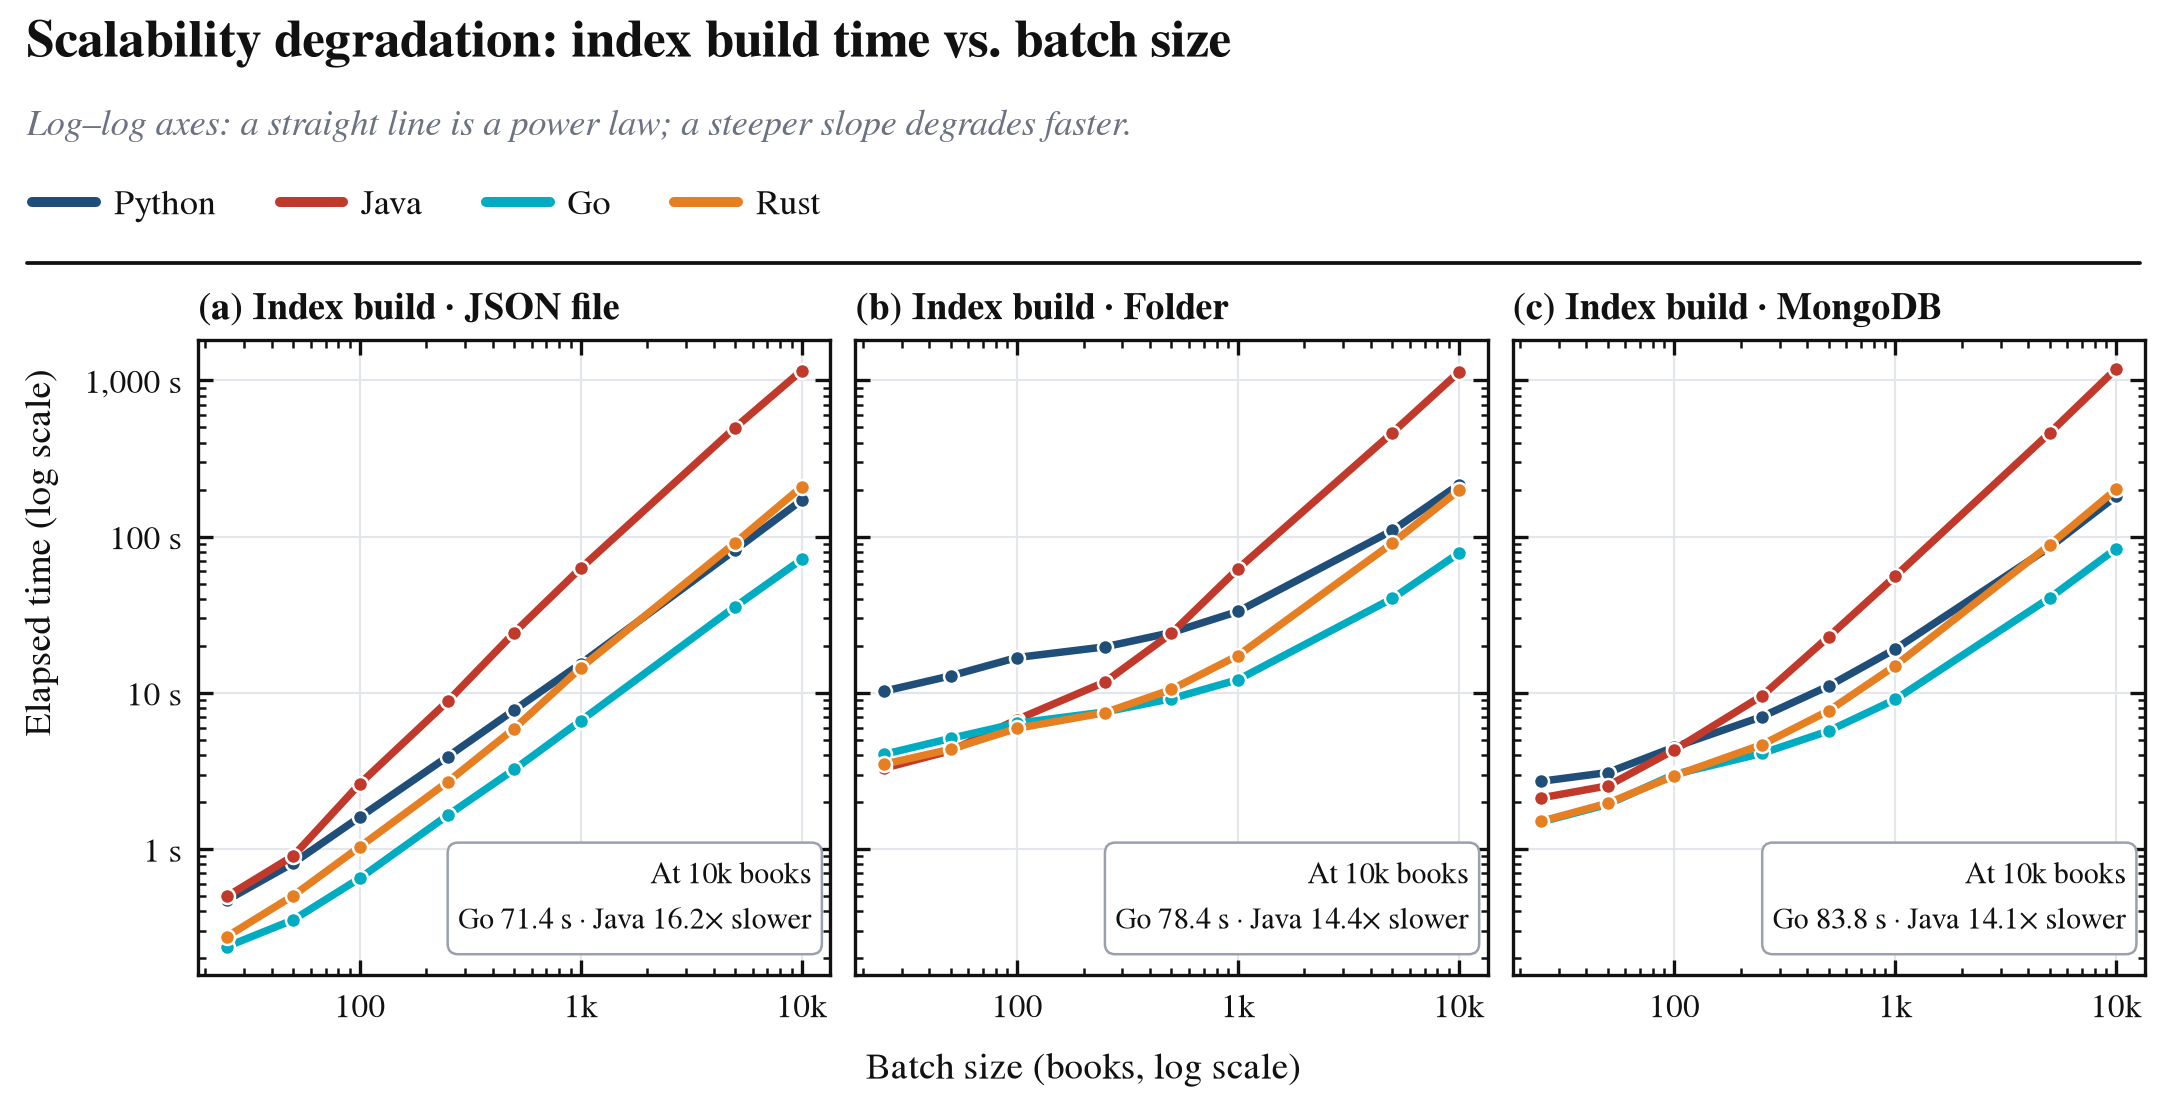
\includegraphics[width=0.94\textwidth]{scalability/scalability_elapsed.png}
        \caption{Build elapsed time versus batch size (log--log), mean of
        5 repetitions up to 1{,}000 books, 3 at 5{,}000 and 2 at 10{,}000
        (\texttt{scalability.csv}).}
        \label{fig:scalability-elapsed}
    \end{minipage}\hfill
    \begin{minipage}[t]{0.48\textwidth}
        \centering
        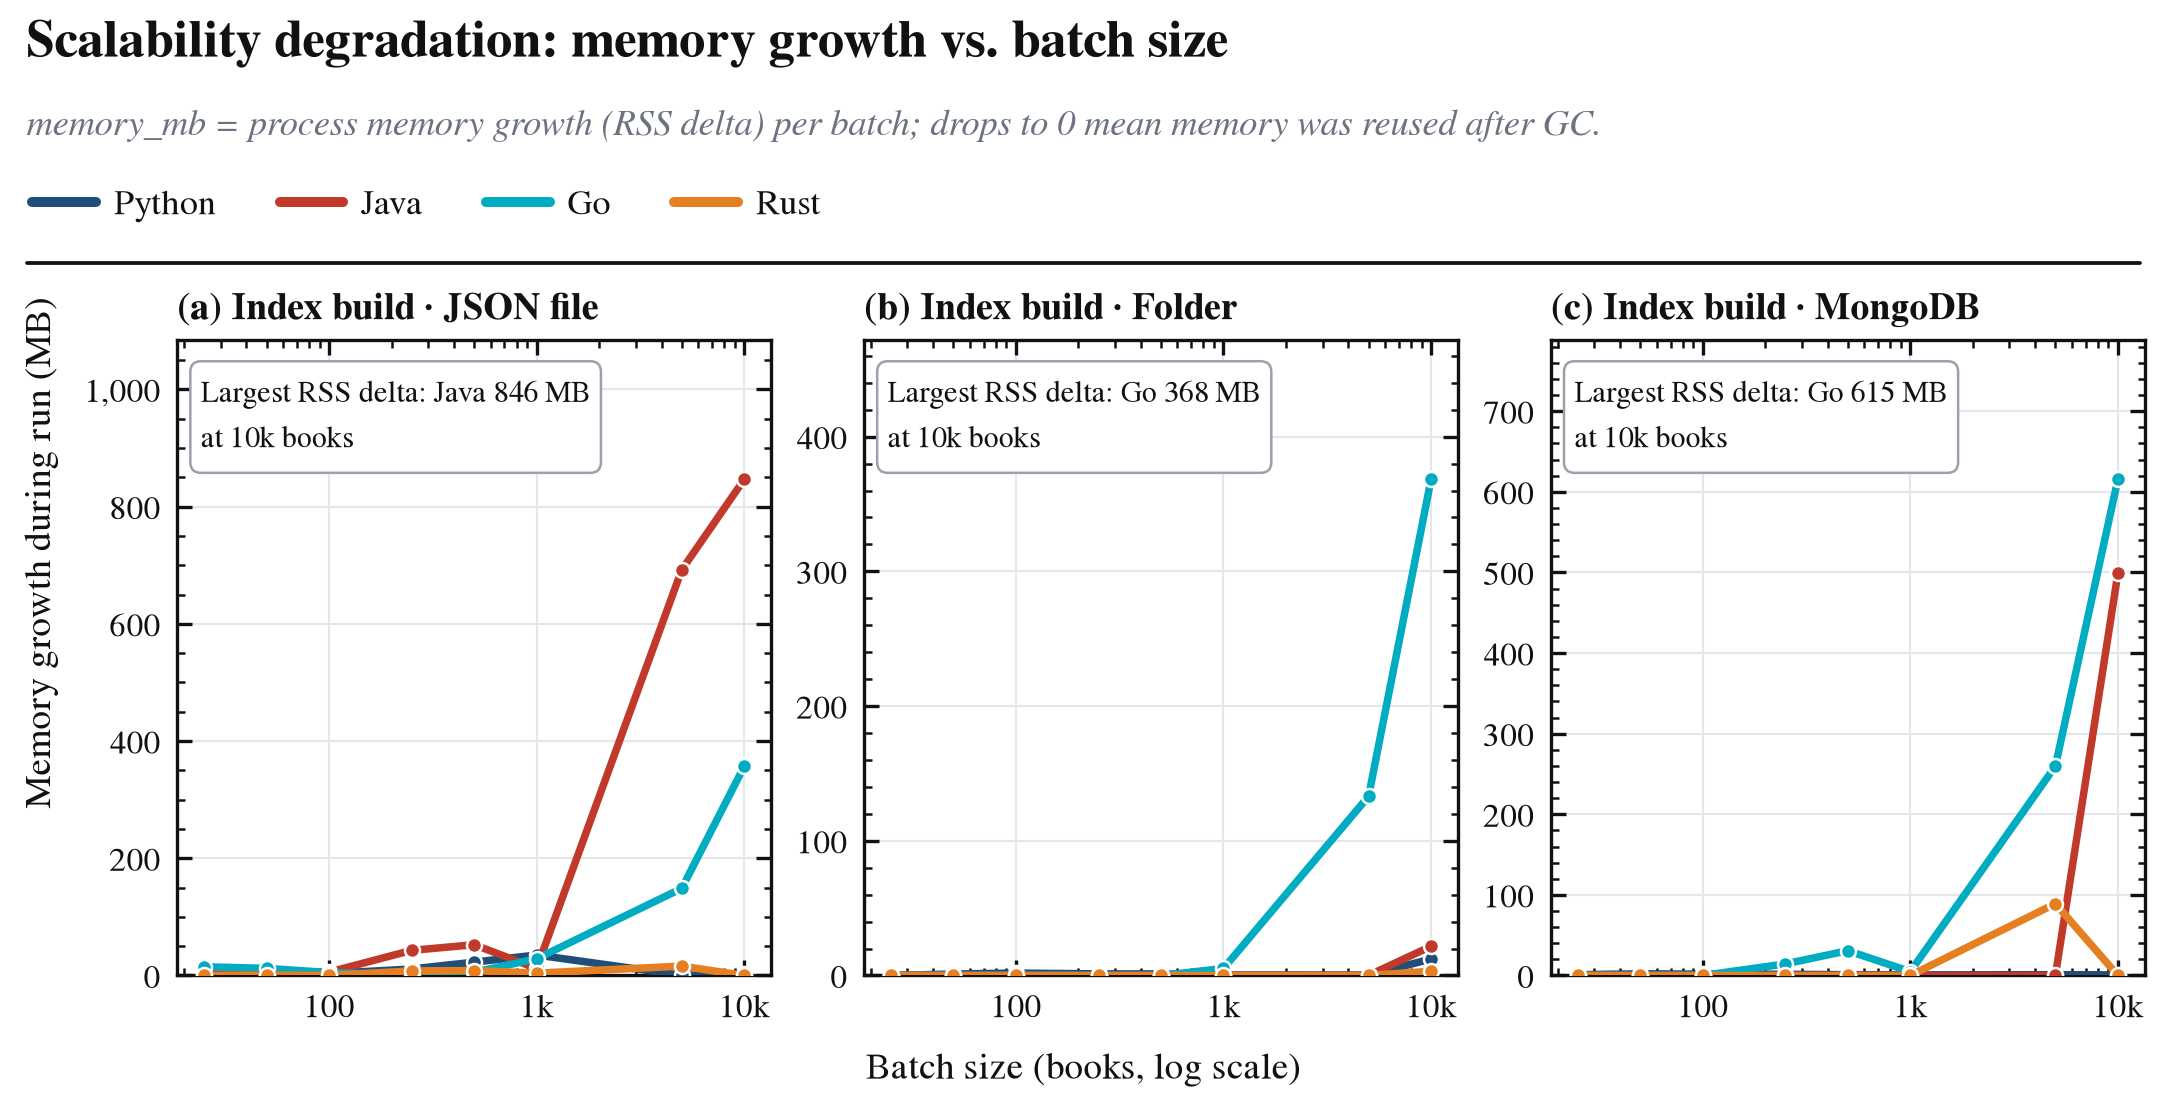
\includegraphics[width=0.94\textwidth]{scalability/scalability_memory.png}
        \caption{Memory growth versus batch size: \textbf{memory\_mb is the
        RSS delta per batch} in MiB, negative deltas reported as 0
        (\cref{tab:metrics}); the callout ``Largest RSS delta'' is the
        largest plotted delta, \emph{not} a process peak
        (\texttt{peak\_rss\_mb}). The subtitle's ``reused after GC'' is one
        possible reason for a zero, not a measured one.}
        \label{fig:scalability-memory}
    \end{minipage}
\end{figure}

\paragraph{Where the build time goes.}
At 10{,}000 books Go built every structure fastest (JSON 71.4~s, folder
78.4~s, MongoDB 83.8~s), followed by Python (170.9--215.3~s) and Rust
(198.1--208.1~s); Java took 1{,}130--1{,}185~s, 14--16$\times$ Go. Two
observations locate the bottleneck. First, within each implementation the
three structures cost nearly the same at 10{,}000 books (within 5\% in Rust
and Java, 17\% in Go, 26\% in Python) although they write very different
artefacts: at this size the build is dominated by the in-memory postings
construction that all three structures share, not by the storage back end.
The back end dominates at small batches instead, where the folder index pays
a fixed cost of one file per term (Python: 10.3~s at 25 books against
0.47~s for the JSON file). Second, the growth rates differ. Between 1{,}000
and 10{,}000 books the log--log slope is 0.81--1.05 for Python and Go,
1.06--1.16 for Rust and 1.26--1.33 for Java, so Java's JSON build grows from
20~ms per book at 25 books to 115~ms per book at 10{,}000, while Go's stays
between 6.5 and 9.5~ms per book.

\paragraph{Why the ports differ: three postings builders.}
The equivalence gate (\cref{sec:equivalence}) guarantees identical postings,
not identical data structures, and the source code shows three strategies
for the same output. The Go port appends a book ID to a term's slice after
an $O(1)$ check of the last element and sorts each slice once at the end. The
Rust port performs a hash lookup and a binary search into the growing
postings vector for every token occurrence. The Java port inserts every token
occurrence into a \texttt{TreeSet<Integer>}, allocating a boxed integer and
a tree node per posting, and copies each set into an \texttt{ArrayList} at
the end; all three Java structures build through this one method, which is
why their times coincide. The isolated \texttt{build\_postings} step over the
100-book corpus follows the same order (Go 0.57~s, Rust 0.88~s, Java 3.07~s;
not recorded by the Python harness), and Java's allocation-heavy strategy is
consistent with its super-linear growth, with process peaks of
5{,}000--5{,}763~MiB under a 5~GiB heap limit, and with the instability of
its JMH \texttt{buildPostings} score (\cref{sec:jmh}). That the data
structure rather than the language causes the gap is a hypothesis supported
by the code and the measurements, not one isolated by a controlled
experiment; it identifies the first optimisation target for Stage~2
(\cref{sec:future}).

\paragraph{The 1{,}601 MB figure.}
In an earlier version of this report a batch was said to ``require 1{,}601
MB''. That number was an RSS \emph{delta}, not a memory requirement and not
a process peak. In the current snapshot the largest plotted build delta is
846.5~MiB (Java, JSON file, 10{,}000 books). The largest delta anywhere in
the snapshot is 1{,}463.8~MiB, recorded by Go for one single-book update of
the 10{,}000-book JSON index (\texttt{benchmarks.csv}), an operation that
loads the whole index, merges one book and rewrites the file. Go's runtime
statistics for that operation show a heap growth of 1{,}267.7~MiB and
3{,}504~MiB allocated in total (\texttt{memstats.csv}), so the delta reflects
real allocation by the update. All four harnesses clamp negative deltas to
zero: a delta of 0 means the resident set did not grow, not that the
operation allocated nothing.

\paragraph{Peak RSS is a high-water mark.}
\texttt{peak\_rss\_mb} is the largest resident set observed while an
operation ran, sampled every \fixed{50}~ms, in a process that has already run
every earlier phase. Runtimes and allocators rarely return memory to the
operating system, so the series behaves as a high-water mark: Rust's peak
stays at 1{,}035.9--1{,}042.3~MiB across all eight folder builds, and Python
reports 3{,}411--3{,}616~MiB peaks for single-book updates of 25- to
1{,}000-book indexes, memory retained from the 10{,}000-book builds that ran
before them. A peak therefore cannot be attributed to the operation in its
row, and the earlier reading ``a peak well above its delta is the spike'' is
withdrawn. As a capacity observation only: the highest peaks were
7{,}304~MiB (Python, folder build of 10{,}000 books), 5{,}763~MiB (Java),
4{,}805~MiB (Go) and 2{,}981~MiB (Rust), on a virtual machine with
9{,}945~MiB of visible memory that also hosted \texttt{mongod}; Python's
peak is 73\% of it.

\paragraph{RAM spikes and garbage collection.}
The only direct collector evidence is Go's runtime record
(\texttt{memstats.csv}). Tokenising the 100-book corpus allocated 616~MiB
over 10 collections, and the 10{,}000-book JSON update allocated
3{,}504~MiB over 2 collections while its in-use heap reached 3{,}837~MiB;
with a single scheduler thread (\texttt{GOMAXPROCS=1}) these collections run
on the measured core. No GC log exists for Java, and recording one with
\texttt{-Xlog:gc} is the cheapest test of the collector hypothesis of
\cref{sec:refactor-effect}.

\subsection{Structures compared}
\label{sec:index-structures}

\paragraph{Where the bytes go.}
The repository also carries an interactive sankey diagram of the storage
breakdown (\texttt{charts/sankey/storage\_sankey.html}, generated by
\texttt{storage\_sankey.py} from \texttt{disk\_usage.csv}) that traces the
corpus bytes from datalake files into each index component; the static
figures of this report quote the same numbers
(\cref{tab:datalake-storage,tab:index-footprint}).

\paragraph{Query latency.}
Every structure answers the \fixed{30} shared queries, \fixed{5} times each
(\fixed{150} samples), on the index left by the 10{,}000-book build. Loading
the JSON file into memory is timed separately (\texttt{load\_json\_index}:
3.7~s Rust, 8.8~s Go, 16.7~s Java; not recorded by the Python harness) and
excluded from the query time. The ordering is the same in all four
implementations (\cref{fig:latency}): the in-memory JSON index is fastest
(0.64--2.68~ms mean), the folder index, which opens one small file per term,
second (1.01--3.84~ms), and MongoDB, which pays a round trip to the server
per term, slowest (4.25--8.31~ms, 1.3--4.8$\times$ the folder index). The
MongoDB means of Python, Go and Rust lie within 4.25--4.97~ms, consistent
with a cost dominated by the server round trip rather than by the client
language. Java's MongoDB mean is inflated by a tail of slow samples
(standard deviation 28.6~ms, maximum 348~ms), which we attribute, as a
hypothesis, to the driver's background threads and the collector sharing the
single pinned core. For every structure and language the standard deviation
is close to the mean: the 30 queries differ widely in cost (a query with an
absent term answers in microseconds), so the mean summarises a mixed
workload, and per-query medians and 95th percentiles are needed before any
latency claim finer than this ordering.

\paragraph{On-disk footprint.}
\Cref{tab:index-footprint} reports the state after the update phase (a
1{,}000-book base plus five single-book additions), which is when the harness
measures it; the 100-book and 10{,}000-book states were not measured.

\begin{table}[htbp]
    \centering
    \caption{Index footprint after the update phase (\texttt{disk\_usage.csv};
    apparent sizes in MiB).}
    \label{tab:index-footprint}
    \begin{tabular}{@{}lccc@{}}
        \toprule
        Structure & Size (MiB) & Files & Directories \\
        \midrule
        JSON file & 75.92 & 1 & 0 \\
        Folder & 42.13 & 106{,}479 & 26 \\
        MongoDB (\texttt{collStats storageSize}) & 5.4--29.6 & --- & --- \\
        \bottomrule
    \end{tabular}
\end{table}

The JSON and folder figures are byte-identical in the four implementations,
as equivalence predicts. The folder figure is an apparent size: at a 4~KiB
block size its 106{,}479 files cannot occupy less than 415.9~MiB of allocated
space, so on a block-based filesystem the folder index is likely the most
expensive structure rather than the cheapest (allocation was not measured).
For MongoDB the client-side file scan is meaningless, so the server's
\texttt{collStats storageSize} is read instead; the collection is dropped and
re-created before every build, in every language. Even so, identical logical
content yields 5.4~MiB (Go), 13.1 (Java), 16.1 (Rust) and 29.6~MiB (Python).
One plausible cause is that \texttt{storageSize} reflects what the storage
engine has written by its last checkpoint, so it depends on when the
statistic is read; we have not verified this. The MongoDB size is therefore
reported, not compared, and no footprint conclusion rests on it.

\subsection{Incremental updates}
\label{sec:index-updates}

Construction cost and update cost are different questions, so updates are
measured separately (\cref{fig:updates}). A base index of \fixed{25, 50,
250, 500, 1000} books is built untimed; then five single-book additions with
fresh synthetic IDs, which cannot collide with the base, are timed one by
one, and their mean is plotted. Every added book carries the same tokens,
computed before timing starts, so tokenisation is not part of the update
time and each addition merges IDs into existing terms without creating new
ones.

\begin{figure}[htbp]
    \centering
    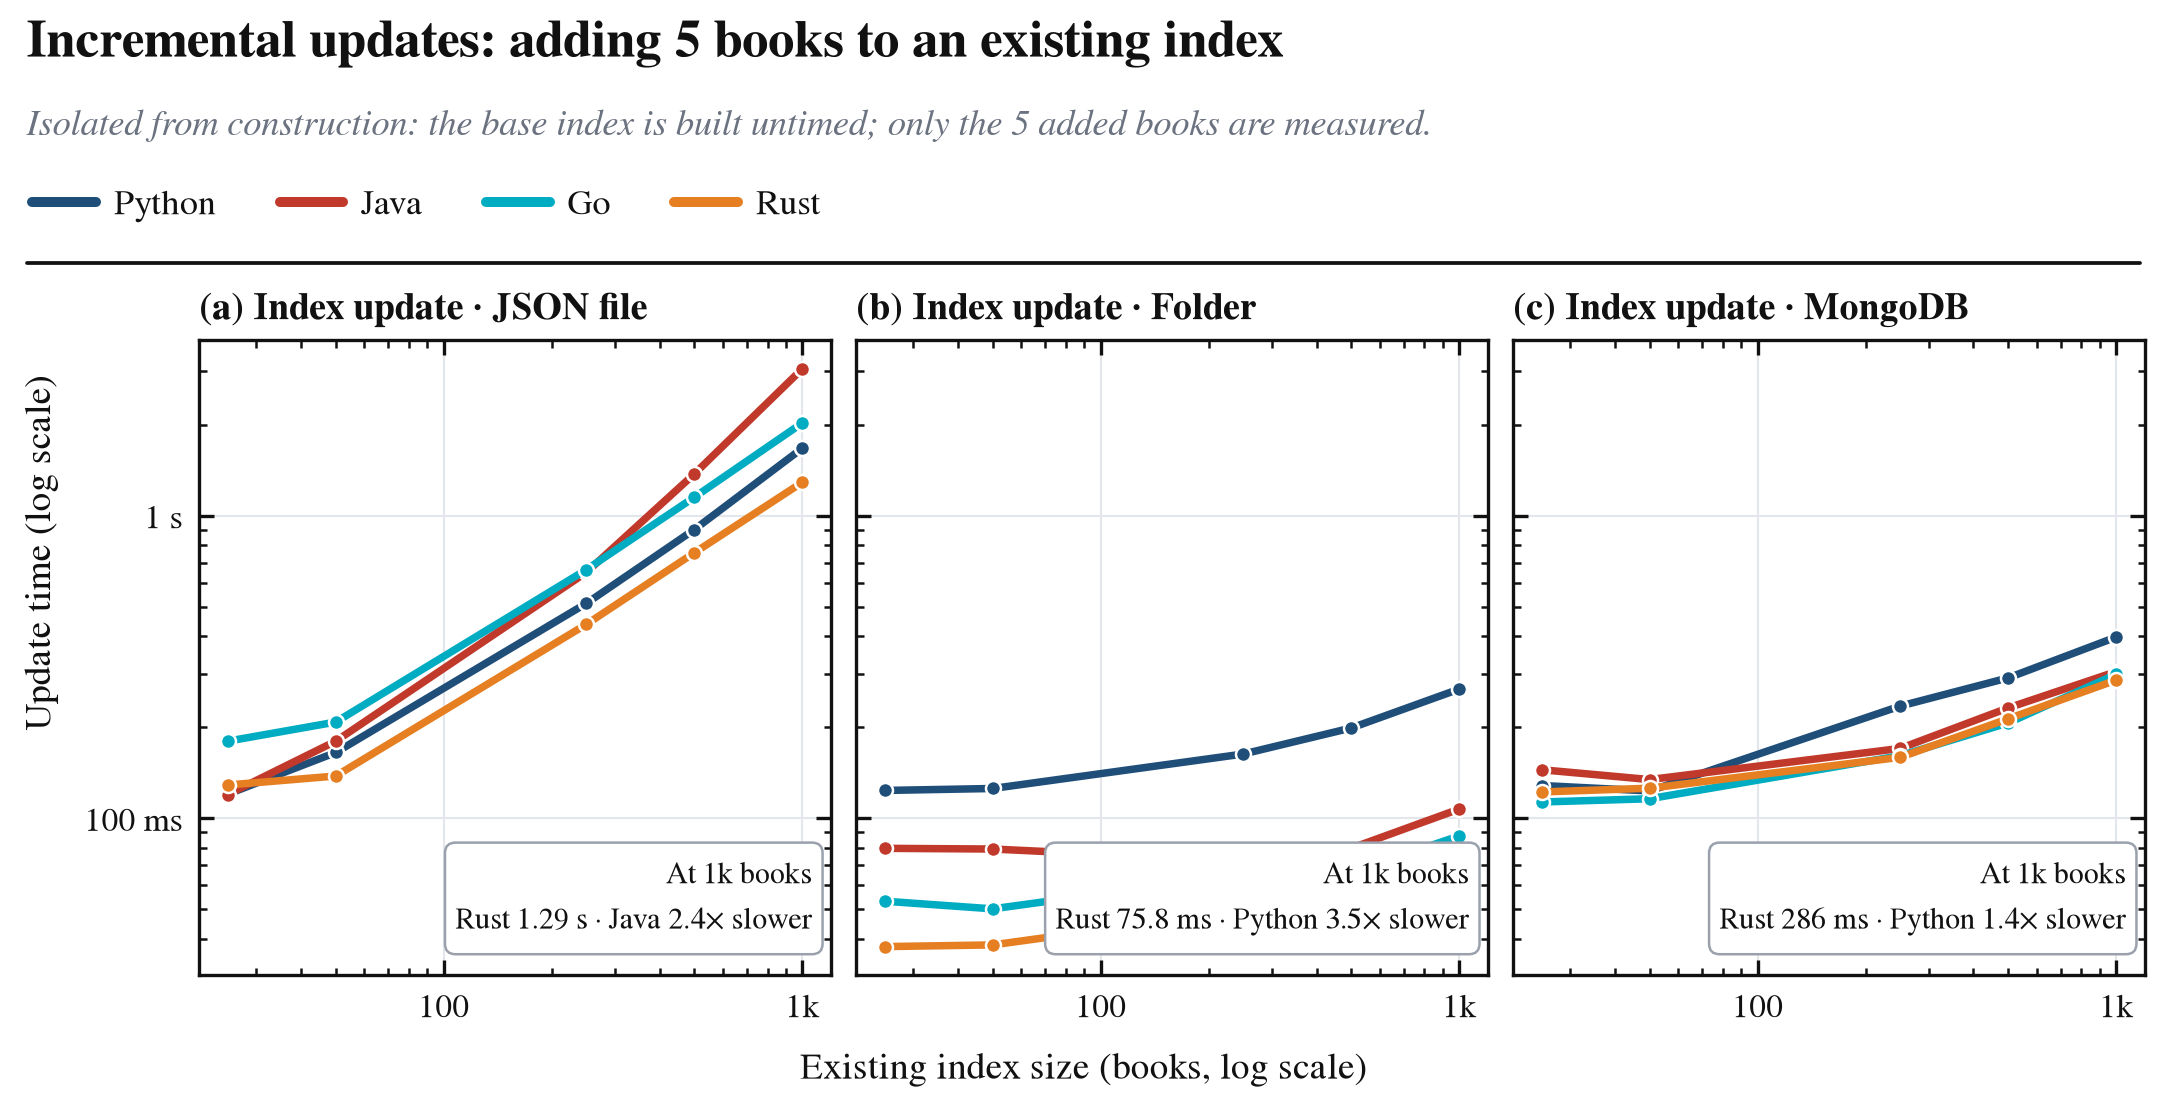
\includegraphics[width=0.72\textwidth]{scalability/scalability_updates.png}
    \caption{Incremental update time versus base index size, isolated from
    construction (\texttt{updates.csv}). Each point is the mean of five
    single-book additions; the ``5 books'' in the figure title are those
    five repetitions, not one five-book batch.}
    \label{fig:updates}
\end{figure}

\paragraph{The O(1) claim.}
The earlier report said MongoDB updates were ``O(1)''. The operation is
\texttt{update\_book}: one upsert per distinct term of the added book, sent
as a single unordered bulk write in all four ports since the current
snapshot. Each upsert runs an update pipeline (\texttt{\$setUnion} followed
by \texttt{\$sortArray}) that rebuilds and re-sorts that term's \emph{whole}
postings array, so the cost depends on the number of terms in the added book
\emph{and} on the postings length of those terms, which grows with the index.
The measurements agree. From base 25 to 1{,}000 the mean update time grew
10.0--25.5$\times$ for the JSON file, 1.35--2.16$\times$ for the folder index
and 2.11--3.09$\times$ for MongoDB. One further single-book update per
structure was timed on the 10{,}000-book index left by the build sweep
(\texttt{benchmarks.csv}, one sample each): JSON 13.1--28.6~s, folder
0.39--1.77~s, MongoDB 2.64--2.92~s. From base 1{,}000 to 10{,}000 the
MongoDB update grew 7.3--9.2$\times$ for a $10\times$ larger base, close to
linear, as expected when the corpus is repeated and a term's postings array
grows in proportion to the base. No structure showed constant update cost;
the O(1) claim is withdrawn and replaced by these curves, and no behaviour is
asserted beyond the measured range (\cref{sec:limitations}).

\paragraph{Which structure updates fastest.}
The folder index had the lowest update time in 18 of the 20
language--base-size points; both exceptions are Python at the smallest bases,
where the JSON file (base 25) and MongoDB (base 50) were 3\% and 2\% faster.
At base 1{,}000 it took 76--267~ms, against
286--397~ms for MongoDB and 1.29--3.06~s for the JSON file. Two
qualifications apply. First, durability is not equal across structures: the
JSON file is written through a temporary file, \texttt{fsync} and rename,
whereas every port rewrites the folder index's term files with plain,
unsynchronised writes, and no port requests more than MongoDB's default
write concern. Part of the folder index's advantage is therefore paid for
with weaker crash guarantees. Second, the MongoDB server runs in its own,
unpinned container, so its share of the work is not bounded by the client's
single-core budget; during the base-10{,}000 update the client itself used
0.4--6.8\% CPU, waiting on the server.

\subsection{Memory and disk of the MongoDB structure}
\label{sec:index-memory}

All client-side memory series (\texttt{memory\_mb}, \texttt{peak\_rss\_mb})
describe the benchmark process only, so \texttt{mongod}'s resident memory is
\emph{not} included in any client figure. The server's cost appears instead
as its own storage, measured through \texttt{collStats storageSize} on the
benchmark database (\texttt{search\_engine\_benchmark}), and as the extra
process a deployment must run. Any capacity statement about MongoDB in this
report refers to that measured size at the measured corpus, plus the
unmeasured server memory, which is listed as a limitation. The server's CPU
is not measured either, and its container has no CPU limit
(\texttt{docker-compose.yml}), so MongoDB-backed phases receive server-side
compute outside the single-core budget of the client
(\cref{sec:host}).

\section{JMH Micro-Benchmarks (Java only)}
\label{sec:jmh}

The end-to-end harness measures whole operations. To see where the Java
implementation spends its time inside those operations, the port carries
four JMH micro-benchmarks over its hot paths
(\texttt{multilang\_ports/java/src/main/java/microbench/}).

\paragraph{Configuration.}
JMH 1.37 on OpenJDK 21.0.12.1, average-time mode, 1 thread, 1 fork, 5+5
iterations of 1~s (warm-up and measurement), GC profiler enabled; the harness
runs on OpenJDK 17 via \texttt{mvn exec:java} --- only the shaded jar targets
21. Raw JSON: \texttt{benchmarks\_\allowbreak results/java/\allowbreak jmh\_\allowbreak results.json},
produced by \texttt{multilang\_\allowbreak ports/java/\allowbreak run\_\allowbreak jmh.sh}.

\begin{table}[htbp]
    \centering
    \caption{JMH results (average time, 1 fork, 5+5 iterations of 1 s).}
    \label{tab:jmh}
    \begin{tabular}{@{}llr@{}}
        \toprule
        Micro-benchmark & Workload & Score \\
        \midrule
        \texttt{TokenizeBenchmark.tokenizeBook} & one sample book & 580.6 $\mu$s/op \\
        \texttt{PostingsBenchmark.buildPostings} & 10 books & 133.5 ms/op \\
        \texttt{PostingsBenchmark.buildPostings} & 100 books & 1853.0 ms/op \\
        \texttt{JsonIndexBenchmark.serializeIndex} & 100-book index & 500.6 ms/op \\
        \texttt{JsonIndexBenchmark.parseIndex} & 100-book index & 114.3 ms/op \\
        \texttt{QueryBenchmark.intersectQuery} & two-term intersection & 2.8 $\mu$s/op \\
        \bottomrule
    \end{tabular}
\end{table}

\paragraph{How these numbers may be used.}
They explain the \emph{internal} split of one Java operation (for example,
serialising the JSON index dominates parsing it by roughly
4.4$\times$), which helps attribute the end-to-end Java bars of
\cref{sec:index}. They are \textbf{evidence about the Java port only}: JMH's
forked-JVM warm-up protocol is deliberately \emph{not} applied to the other
languages, so no JMH number is ever placed next to a Python, Go or Rust
measurement in this report. The cross-language figures of
\cref{sec:language-performance} all come from the common harness of
\cref{sec:methodology}.

\section{Conclusions and Final Architecture Selection}
\label{sec:conclusions}

\paragraph{What the measurements support.}
On the host of \cref{tab:host}, over the \fixed{100}-book corpus and the
\fixed{30}-query workload, the tournament measured the following:

\begin{itemize}
    \item The four implementations are behaviourally identical on this
    workload (byte-identical canonical outputs, \cref{sec:equivalence}), so
    the cross-language differences below compare the same work.
    \item On write throughput and datalake lookup, the measured spread
    between implementations is \pending{throughput/lookup summary}.
    \item On index build time and query latency, \pending{build/query
    summary}; on incremental updates over the measured base sizes,
    \pending{update summary}.
    \item On-disk footprint is dominated by the corpus itself; the storage
    overhead of the three index structures over the same corpus is
    \pending{index storage summary} (\cref{sec:index-memory}).
    \item Recovery after a documented interruption resumed with
    \pending{0} duplicated and \pending{0} lost books in every layout
    (\cref{tab:recovery}).
\end{itemize}

\paragraph{Selection for Stage 2.}
Within the tested corpus, workload and host, the group selects
\textbf{Java with the MongoDB index structure} for Stage 2. The reasoning is
scoped to the evidence: MongoDB showed \pending{measured update and space
behaviour} at the measured sizes, its server-side footprint was measured
separately (\texttt{collStats}), and the Java port's end-to-end numbers were
supported by JMH attribution. This is a choice \emph{for the Stage 2
workload}, not a claim that Java is universally faster or that MongoDB is
the only scalable storage: at the measured scale, the file-based structures
were competitive on several axes, and behaviours that matter at larger
scale --- sharding, replication, concurrency, multi-gigabyte indexes ---
were \emph{not measured here} and remain open questions
(\cref{sec:limitations}).

\paragraph{Language-wide claims.}
Nothing in this report supports a statement of the form ``language X is
faster than language Y''. The measured objects are four implementations,
written by this team, of one pipeline, on one corpus, on one machine, in one
continuous run. Statements such as ``Go's allocator showed the lowest RSS
growth in this workload'' are observations; ``Go uses less memory'' is a
hypothesis this experiment cannot test. Where the data was ambiguous, the
report says so rather than picking a narrative.

\subsection{Future Improvements}
\label{sec:future}

\begin{itemize}
    \item Repeat the tournament on bare metal and on Linux natively to
    separate runtime effects from WSL2's virtualisation.
    \item Extend the corpus by an order of magnitude to observe where the
    measured curves bend (the current 10{,}000-book batch reuses a
    100-book corpus, \cref{sec:workload}).
    \item Measure concurrency (multiple query clients) for the Stage 2
    serving layer, where it will actually be used.
    \item Add a memory-profiled MongoDB run that accounts the server's RSS
    alongside the client's, for a true capacity figure.
\end{itemize}

\section{Limitations}
\label{sec:limitations}

Every observed difference could partly be an artefact of the following
factors. They are listed so readers can weigh the results accordingly.

\paragraph{Machine.}
One laptop-class host (i7-10750H, 8 GB RAM), under WSL2 virtualisation, with
an NTFS-backed filesystem. CPU frequency scaling, thermal throttling and the
hypervisor layer affect all languages, but not necessarily equally. Every
timed harness phase is pinned to a single logical core with \texttt{taskset}
(\cref{sec:host}), which bounds the CPU budget but is no performance governor
and no bare metal: neighbouring work still shares that core.

\paragraph{Runtime.}
The Java harness and JMH both run on OpenJDK 21 (the harness through
\texttt{mvn exec:java}, whose own JVM overhead is outside the timed regions
but shares the machine; JMH in a shaded jar). Python runs on 3.14, Go 1.27,
Rust 1.99: these are current
versions, not long-term-stability comparisons. Only Java receives warm-up
(\cref{sec:warmup}); the other languages are measured from cold start, which
is the honest default for them but is itself a protocol choice.

\paragraph{Cache state.}
The OS page cache is never dropped between phases, so a file read twice in
one phase may be served from RAM. All languages in a phase share the same
state, but phases are not independent of the ones before them. MongoDB's
internal cache (WiredTiger) is likewise warm after the first build.

\paragraph{Workload.}
The corpus is \fixed{100} books (\fixed{61.4} MB); the scalability
builds reach 10{,}000 ``books'' by repeating that corpus, so index size
grows but term diversity does not. The datalake experiments stay at the same \fixed{100} books: they compare
directory structures on identical work, and growing them would mean
downloading thousands more books (breaking the frozen artifact) or
duplicating files (measuring nothing new) --- no datalake scaling curve was
measured. Queries are \fixed{30} fixed lines; they are
representative of the assignment but not sampled from a query log.
Results may reorder on corpora with different term distributions.

\paragraph{Timing and statistics.}
Elapsed times are wall-clock on a shared host where only the CPU budget is
pinned (\cref{sec:host}): neighbouring
processes (including \texttt{mongod} and the sampling threads) inject
jitter, visible as non-zero \texttt{stdev\_seconds}. One tournament run
produces the committed snapshot; there is no second run to quantify
run-to-run variance. No outliers are trimmed and no phase is repeated for a
better result.

\paragraph{Measurement boundaries.}
Client RSS excludes the MongoDB server by construction
(\cref{sec:index-memory}); its storage is measured via \texttt{collStats},
its memory is not. The download probe is ten sequential requests per round
over one pooled connection, repeated in five interleaved rounds, so its
rate reflects latency more than bandwidth. CPU percentage is process CPU
over wall clock; the pinned harness phases cannot exceed 100.

\paragraph{Unmeasured behaviours.}
Not exercised at all: concurrent readers and writers, indexes far beyond the
measured batches, MongoDB replication/sharding, crash recovery of the
database itself, and the Stage 2 serving path. Conclusions in
\cref{sec:conclusions} do not extend to them.

\section{Reproducibility}
\label{sec:reproducibility}

Every figure in this report is reproducible from the repository at a single
identified revision. The full protocol is documented in
\texttt{REPRODUCING.md}; the short version follows.

\paragraph{One command.}
\texttt{./scripts/run\_tournament.sh} runs five phases in order and refuses
to time anything before equivalence passes:

\begin{enumerate}
    \item \textbf{equivalence} --- cross-language canonical files, compared
    byte for byte (\texttt{equivalence\_\allowbreak report.json});
    \item \textbf{benchmarks} --- Go, Rust, Java (+JMH) and Python suites,
    each writing its CSVs under
    \texttt{benchmarks\_\allowbreak results/\allowbreak <language>/};
    \item \textbf{verify} --- schema check of every CSV
    (\texttt{scripts/\allowbreak verify\_\allowbreak format.py});
    \item \textbf{environment} --- host, runtimes and Git revision in
    \texttt{benchmarks\_\allowbreak results/\allowbreak environment.txt};
    \item \textbf{charts} --- \texttt{src/\allowbreak visualizations/\allowbreak main.py} renders \texttt{charts/}.
\end{enumerate}

There is no resume: a failed run restarts clean, so the committed snapshot
always comes from one continuous execution.

\paragraph{Chart-to-artifact map.}
\Cref{tab:chart-map} links every figure to its script (all chart scripts
live under \texttt{src/\allowbreak visualizations/\allowbreak modules/}), its raw results and its
configuration.

\begin{table}[htbp]
    \centering
    \small
    \caption{Where each figure comes from.}
    \label{tab:chart-map}
    \begin{tabularx}{\textwidth}{@{}llX@{}}
        \toprule
        Figure & Script & Raw results \\
        \midrule
        \cref{fig:radar} & \texttt{radar\_chart.py} & all of \texttt{benchmarks\_results/} \\
        \cref{fig:throughput} & \texttt{throughput\_charts.py} & \texttt{\*/throughput.csv}, \texttt{\*/benchmarks.csv} \\
        \cref{fig:latency} & \texttt{latency\_charts.py} & \texttt{\*/statistics.csv} \\
        \cref{fig:scalability-elapsed,fig:scalability-memory,fig:updates} & \texttt{scalability\_charts.py} & \texttt{\*/scalability.csv}, \texttt{\*/updates.csv} \\
        Sankey (interactive HTML) & \texttt{storage\_sankey.py} & \texttt{\*/disk\_usage.csv} \\
        \cref{tab:jmh} & \texttt{multilang\_ports/java/run\_jmh.sh} & \texttt{java/jmh\_results.json} \\
        \bottomrule
    \end{tabularx}
\end{table}

\paragraph{Revision.}
The Git commit that produced the committed snapshot is recorded inside
\texttt{benchmarks\_\allowbreak results\_\allowbreak environment.txt} together with the host and
runtime versions of \cref{tab:host}. Checking out that commit and re-running
the command above reproduces the pipeline; the raw numbers will differ in
their last digits (shared-host jitter, \cref{sec:limitations}), but the
ordering and the equivalence digests are stable.

\section{Correction Comment Matrix}
\label{sec:comment-matrix}

\begin{center}
\footnotesize
\renewcommand{\arraystretch}{0.80}
\begin{longtable}{@{}lp{4.2cm}p{11.2cm}@{}}
    \caption{Correction comments mapped to the place that answers each one.}\label{tab:comment-matrix}\\
    \toprule
    \# & Topic & Where it is addressed \\
    \midrule
    \endfirsthead
    \toprule
    \# & Topic & Where it is addressed \\
    \midrule
    \endhead
    1 & Scope language/storage claims to the workload &
    \cref{sec:introduction,sec:conclusions}: scoped to corpus, host, workload. \\
    2 & Host, runtimes, parameters, download concurrency &
    \cref{tab:host,tab:workload,sec:environment-state}: downloads sequential. \\
    3 & RSS-delta definition, 1{,}601 MB, O(1) MongoDB &
    \cref{sec:index-scalability}: delta vs peak (846.5/1{,}463.8~MiB);
    \cref{sec:index-updates}: O(1) replaced. \\
    4 & Pipeline diagram of the three layers &
    \cref{fig:pipeline}: TikZ, layers, data movement, durable writes. \\
    5 & Radar productivity axis, ``Peak'' callout &
    \cref{sec:radar,fig:scalability-memory}: qualitative score stated; callout renamed. \\
    6 & Discovery, storage overhead, recovery observations &
    \cref{sec:datalake-discovery,sec:datalake-storage,sec:datalake-recovery}: CSVs. \\
    7 & Normalisation/metadata rules, postings examples, all languages &
    \cref{sec:normalisation,sec:metadata-contract,sec:equivalence-languages}: rules and example. \\
    8 & Link charts to script, config, raw results, revision &
    \cref{tab:chart-map,sec:provenance}; \texttt{environment.txt}. \\
    9 & Limitations section & \cref{sec:limitations}. \\
    10 & Do not call MongoDB ``the only scalable choice'' &
    \cref{sec:conclusions}: selection scoped to Stage~2. \\
    11 & Delta vs peak RSS, RAM-spike/GC evidence, O(1) variable &
    \cref{sec:index-scalability}: peak sampling, Go \texttt{memstats};
    \cref{sec:index-updates}. \\
    12 & Compare metadata, terms, postings, answers; equivalence first &
    \cref{sec:equivalence}: gates before timing, byte-identical. \\
    13 & Record host, runtimes and concurrency per language, align or restrict &
    \cref{tab:host,tab:workload,tab:coverage,sec:warmup}: identical parameters. \\
    14 & Corpus, operation and timing boundaries behind plots &
    \cref{sec:workload,sec:timing-boundaries,sec:coverage}. \\
    15 & Reinterpret RAM/timing; language explanations as hypotheses &
    \cref{sec:conclusions,sec:throughput-latency}: reading rule. \\
    16 & Book counts, sizes, timing start/stop for write and download &
    \cref{sec:timing-boundaries,sec:datalake-throughput}. \\
    17 & Discovery of downloaded-but-not-indexed books, same state &
    \cref{sec:datalake-discovery,tab:discovery}: identical state, one sample. \\
    18 & Files, directories, auxiliary state, bytes per layout &
    \cref{sec:datalake-storage,tab:datalake-storage}; \texttt{disk\_usage.csv}. \\
    19 & Directory counts before choosing batches; complement lookup &
    \cref{sec:datalake-storage,sec:index-structures}: counts tie to lookup. \\
    20 & Isolated incremental-update experiment &
    \cref{sec:index-updates,fig:updates}: bases 25--1000, five additions each, one at 10{,}000. \\
    21 & Publish workload and expected answers; cross-structure check &
    \texttt{queries.txt} with \cref{tab:workload}; \cref{sec:equivalence-structures}. \\
    22 & Sampling procedure, processes included, peak RSS, MongoDB server &
    \cref{tab:metrics,sec:index-memory}: 50~ms sampling; server via \texttt{collStats}. \\
    23 & Support MongoDB with measured updates/space; drop O(1) &
    \cref{sec:index-updates,sec:index-memory,fig:updates}; selection on Stage~2
    requirements (\cref{sec:conclusions}). \\
    24 & Demonstrated interruption and resumption with counts &
    \cref{sec:datalake-recovery,tab:recovery}; kill-and-restart in \cref{sec:future}. \\
    25 & Compare IDs, metadata, postings, answers; also after updates &
    \cref{sec:equivalence-structures}: repeated after an update. \\
    26 & Limit Java/MongoDB conclusions; state unmeasured behaviours &
    \cref{sec:conclusions,sec:limitations}. \\
    27 & CPU, RAM, storage, OS, exact runtime versions &
    \cref{tab:host}; \texttt{environment.txt}. \\
    28 & Corpus IDs/sizes, queries, update batch, coverage &
    \cref{tab:workload,tab:coverage}; \texttt{equivalence\_report.json}. \\
    29 & Output preparation, cache state, network, warm-up &
    \cref{sec:environment-state,sec:warmup}: fresh tree, Java-only warm-up. \\
    30 & Sample count, clock, timing boundaries, repetition procedure &
    \cref{tab:metrics,tab:workload,sec:timing-boundaries,sec:uncertainty}. \\
    31 & Exact commands and raw-result locations per chart, revision &
    \cref{sec:reproducibility,tab:chart-map}; \texttt{environment.txt}. \\
    32 & Pipeline quality; Stage 2 search not required &
    No change: search belongs to Stage~2 (\cref{sec:architecture}). \\
    33 & Code quality; no deduction for Stage 2 or optional packages &
    No change: optional dependencies in \texttt{REPRODUCING.md}. \\
    \bottomrule
\end{longtable}
\end{center}


\end{document}
